% nicrainha's color science: a deck for the nicrainha showcase. Its figures
% are the library's own numbers (the gamut slices, r(L*), the n-gons and
% palettes), computed with nicrainha and written in as TikZ coordinates.
\begin{filecontents*}[overwrite]{nicrainha.bib}
@book{cie,
  author = {{CIE}}, title = {Colorimetry}, edition = {Third},
  publisher = {Commission Internationale de l'\'Eclairage},
  note = {CIE 15:2004}, year = {2004}}
@misc{srgb,
  author = {{IEC}}, title = {Multimedia systems and equipment -- Colour
  measurement and management -- Part 2-1: Default {RGB} colour space -- {sRGB}},
  howpublished = {IEC 61966-2-1}, year = {1999}}
@article{bresenham,
  author = {Jack E. Bresenham}, title = {Algorithm for computer control of a
  digital plotter}, journal = {IBM Systems Journal}, volume = {4}, number = {1},
  pages = {25--30}, year = {1965}}
@article{kuhn,
  author = {Harold W. Kuhn}, title = {The {H}ungarian method for the assignment
  problem}, journal = {Naval Research Logistics Quarterly}, volume = {2},
  pages = {83--97}, year = {1955}}
@article{munkres,
  author = {James Munkres}, title = {Algorithms for the assignment and
  transportation problems}, journal = {Journal of the Society for Industrial
  and Applied Mathematics}, volume = {5}, number = {1}, pages = {32--38},
  year = {1957}}
@misc{wcag,
  author = {{W3C}}, title = {Web Content Accessibility Guidelines ({WCAG}) 2.2},
  howpublished = {W3C Recommendation}, year = {2023}}
\end{filecontents*}
\documentclass{nicrainha}
\usepackage{tikz}
\usetikzlibrary{arrows.meta}

\title{nicrainha's color science}
\author{Perceptually even palettes from CIELAB}
\date{November 2026}

\begin{document}
\maketitle

\begin{slide}{One lightness}
  A nicrainha palette is a set of colors that differ only in hue.
  \begin{itemize}
    \item Every color has the same CIELAB lightness $L^*$ \cite{cie}.
    \item The same $L^*$ means the same relative luminance:
      \[ Y = \left(\frac{L^* + 16}{116}\right)^{3} \qquad (L^* > 8). \]
    \item So every color has the same contrast with any gray, black and
      white included.
    \item No color shouts: the palette is even to the eye.
  \end{itemize}
\end{slide}

\begin{slide}{CIELAB in one slide}
  From linear sRGB \cite{srgb} to XYZ (D65), then
  \begin{align*}
    L^* &= 116\, f(Y/Y_n) - 16, \\
    a^* &= 500\, \bigl(f(X/X_n) - f(Y/Y_n)\bigr), \\
    b^* &= 200\, \bigl(f(Y/Y_n) - f(Z/Z_n)\bigr),
  \end{align*}
  \[
    f(t) = \begin{cases}
      t^{1/3} & t > \delta^3, \\
      \dfrac{t}{3\delta^2} + \dfrac{4}{29} & \text{otherwise},
    \end{cases}
    \qquad \delta = \frac{6}{29}.
  \]
  A constant-$L^*$ plane is a slice through the gamut; hue is the angle in it.
\end{slide}

\begin{slide}{The 256-gon}
  Fix $L^*$. On its plane, take the regular 256-gon centered on the gray axis,
  anchored at $-b^*$:
  \[
    v_k = \bigl(L^*,\ r\cos\theta_k,\ r\sin\theta_k\bigr), \qquad
    \theta_k = \frac{3\pi}{2} + \frac{2\pi k}{256}, \qquad k = 0, \dots, 255.
  \]
  Its radius is the largest that keeps every vertex in sRGB:
  \[
    r(L^*) = \min_{k}\ \sup\,\{\, r \ge 0 : v_k(r) \in \text{sRGB} \,\}.
  \]
  Every palette is a subset of these 256 colors.
\end{slide}

\begin{slide}{Inscribed in the gamut}
  \begin{minipage}[c]{0.56\linewidth}
    \centering
    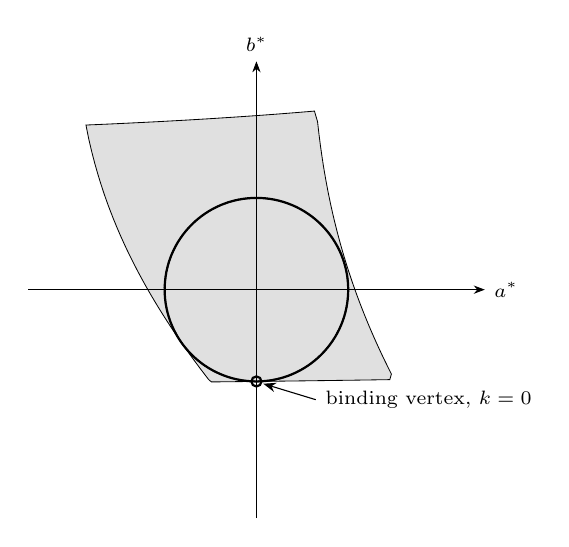
\begin{tikzpicture}[x=0.29mm, y=0.29mm]
    \draw[-{Stealth[length=1.4mm]}, line width=0.3pt] (-100,0) -- (100,0) node[right, font=\scriptsize] {$a^*$};
    \draw[-{Stealth[length=1.4mm]}, line width=0.3pt] (0,-100) -- (0,100) node[above, font=\scriptsize] {$b^*$};
    \fill[fill opacity=0.12] (43.15,0) -- (42.62,1.49) -- (42.11,2.94) -- (41.62,4.37) -- (41.15,5.78) -- (40.69,7.17) -- (40.24,8.55) -- (39.8,9.92) -- (39.37,11.29) -- (38.95,12.66) -- (38.53,14.02) -- (38.12,15.4) -- (37.71,16.79) -- (37.31,18.2) -- (36.9,19.62) -- (36.5,21.07) -- (36.1,22.56) -- (35.69,24.08) -- (35.29,25.64) -- (34.88,27.25) -- (34.46,28.92) -- (34.04,30.65) -- (33.61,32.46) -- (33.18,34.35) -- (32.73,36.35) -- (32.27,38.46) -- (31.81,40.71) -- (31.32,43.11) -- (30.83,45.7) -- (30.31,48.51) -- (29.78,51.58) -- (29.22,54.96) -- (28.65,58.73) -- (28.04,62.99) -- (27.42,67.87) -- (26.77,73.55) -- (25.41,78.21) -- (22.35,77.95) -- (19.37,77.71) -- (16.47,77.47) -- (13.62,77.25) -- (10.83,77.03) -- (8.07,76.82) -- (5.36,76.62) -- (2.67,76.42) -- (0,76.23) -- (-2.66,76.04) -- (-5.3,75.86) -- (-7.95,75.68) -- (-10.61,75.5) -- (-13.28,75.33) -- (-15.97,75.16) -- (-18.7,74.98) -- (-21.45,74.81) -- (-24.25,74.64) -- (-27.11,74.47) -- (-30.02,74.3) -- (-33.01,74.13) -- (-36.07,73.96) -- (-39.23,73.79) -- (-42.5,73.61) -- (-45.89,73.44) -- (-49.41,73.26) -- (-53.09,73.08) -- (-56.95,72.89) -- (-61,72.7) -- (-65.28,72.5) -- (-69.82,72.3) -- (-74.66,72.1) -- (-73.47,66.15) -- (-72.16,60.55) -- (-70.8,55.32) -- (-69.41,50.43) -- (-67.99,45.86) -- (-66.58,41.6) -- (-65.17,37.62) -- (-63.77,33.91) -- (-62.4,30.44) -- (-61.06,27.18) -- (-59.75,24.14) -- (-58.47,21.28) -- (-57.23,18.59) -- (-56.02,16.06) -- (-54.85,13.68) -- (-53.71,11.42) -- (-52.61,9.28) -- (-51.54,7.24) -- (-50.5,5.31) -- (-49.48,3.46) -- (-48.5,1.69) -- (-47.54,0) -- (-46.6,-1.63) -- (-45.68,-3.19) -- (-44.78,-4.71) -- (-43.9,-6.17) -- (-43.04,-7.59) -- (-42.19,-8.97) -- (-41.35,-10.31) -- (-40.52,-11.62) -- (-39.7,-12.9) -- (-38.89,-14.16) -- (-38.09,-15.39) -- (-37.29,-16.6) -- (-36.49,-17.8) -- (-35.7,-18.98) -- (-34.91,-20.15) -- (-34.12,-21.32) -- (-33.32,-22.47) -- (-32.52,-23.63) -- (-31.71,-24.78) -- (-30.9,-25.93) -- (-30.08,-27.08) -- (-29.25,-28.24) -- (-28.4,-29.41) -- (-27.54,-30.59) -- (-26.67,-31.78) -- (-25.77,-32.99) -- (-24.86,-34.21) -- (-23.92,-35.46) -- (-22.95,-36.73) -- (-21.96,-38.03) -- (-20.93,-39.37) -- (-19.71,-40.4) -- (-17.98,-40.39) -- (-16.31,-40.37) -- (-14.69,-40.35) -- (-13.11,-40.33) -- (-11.56,-40.32) -- (-10.05,-40.3) -- (-8.56,-40.28) -- (-7.1,-40.27) -- (-5.66,-40.25) -- (-4.23,-40.24) -- (-2.81,-40.22) -- (-1.4,-40.2) -- (0,-40.19) -- (1.4,-40.17) -- (2.81,-40.16) -- (4.22,-40.14) -- (5.64,-40.12) -- (7.07,-40.1) -- (8.52,-40.09) -- (9.99,-40.07) -- (11.48,-40.05) -- (13.01,-40.03) -- (14.56,-40.01) -- (16.16,-39.99) -- (17.8,-39.97) -- (19.49,-39.95) -- (21.23,-39.93) -- (23.04,-39.9) -- (24.92,-39.88) -- (26.88,-39.85) -- (28.94,-39.83) -- (31.09,-39.8) -- (33.37,-39.77) -- (35.78,-39.73) -- (38.33,-39.7) -- (41.07,-39.66) -- (44,-39.62) -- (47.16,-39.57) -- (50.58,-39.52) -- (54.32,-39.46) -- (58.41,-39.4) -- (59.11,-36.94) -- (57.14,-32.99) -- (55.43,-29.47) -- (53.94,-26.31) -- (52.62,-23.43) -- (51.44,-20.78) -- (50.37,-18.33) -- (49.39,-16.05) -- (48.5,-13.91) -- (47.67,-11.89) -- (46.9,-9.97) -- (46.18,-8.14) -- (45.51,-6.4) -- (44.87,-4.72) -- (44.27,-3.1) -- (43.69,-1.53) -- cycle;
    \draw[line width=0.3pt] (43.15,0) -- (42.62,1.49) -- (42.11,2.94) -- (41.62,4.37) -- (41.15,5.78) -- (40.69,7.17) -- (40.24,8.55) -- (39.8,9.92) -- (39.37,11.29) -- (38.95,12.66) -- (38.53,14.02) -- (38.12,15.4) -- (37.71,16.79) -- (37.31,18.2) -- (36.9,19.62) -- (36.5,21.07) -- (36.1,22.56) -- (35.69,24.08) -- (35.29,25.64) -- (34.88,27.25) -- (34.46,28.92) -- (34.04,30.65) -- (33.61,32.46) -- (33.18,34.35) -- (32.73,36.35) -- (32.27,38.46) -- (31.81,40.71) -- (31.32,43.11) -- (30.83,45.7) -- (30.31,48.51) -- (29.78,51.58) -- (29.22,54.96) -- (28.65,58.73) -- (28.04,62.99) -- (27.42,67.87) -- (26.77,73.55) -- (25.41,78.21) -- (22.35,77.95) -- (19.37,77.71) -- (16.47,77.47) -- (13.62,77.25) -- (10.83,77.03) -- (8.07,76.82) -- (5.36,76.62) -- (2.67,76.42) -- (0,76.23) -- (-2.66,76.04) -- (-5.3,75.86) -- (-7.95,75.68) -- (-10.61,75.5) -- (-13.28,75.33) -- (-15.97,75.16) -- (-18.7,74.98) -- (-21.45,74.81) -- (-24.25,74.64) -- (-27.11,74.47) -- (-30.02,74.3) -- (-33.01,74.13) -- (-36.07,73.96) -- (-39.23,73.79) -- (-42.5,73.61) -- (-45.89,73.44) -- (-49.41,73.26) -- (-53.09,73.08) -- (-56.95,72.89) -- (-61,72.7) -- (-65.28,72.5) -- (-69.82,72.3) -- (-74.66,72.1) -- (-73.47,66.15) -- (-72.16,60.55) -- (-70.8,55.32) -- (-69.41,50.43) -- (-67.99,45.86) -- (-66.58,41.6) -- (-65.17,37.62) -- (-63.77,33.91) -- (-62.4,30.44) -- (-61.06,27.18) -- (-59.75,24.14) -- (-58.47,21.28) -- (-57.23,18.59) -- (-56.02,16.06) -- (-54.85,13.68) -- (-53.71,11.42) -- (-52.61,9.28) -- (-51.54,7.24) -- (-50.5,5.31) -- (-49.48,3.46) -- (-48.5,1.69) -- (-47.54,0) -- (-46.6,-1.63) -- (-45.68,-3.19) -- (-44.78,-4.71) -- (-43.9,-6.17) -- (-43.04,-7.59) -- (-42.19,-8.97) -- (-41.35,-10.31) -- (-40.52,-11.62) -- (-39.7,-12.9) -- (-38.89,-14.16) -- (-38.09,-15.39) -- (-37.29,-16.6) -- (-36.49,-17.8) -- (-35.7,-18.98) -- (-34.91,-20.15) -- (-34.12,-21.32) -- (-33.32,-22.47) -- (-32.52,-23.63) -- (-31.71,-24.78) -- (-30.9,-25.93) -- (-30.08,-27.08) -- (-29.25,-28.24) -- (-28.4,-29.41) -- (-27.54,-30.59) -- (-26.67,-31.78) -- (-25.77,-32.99) -- (-24.86,-34.21) -- (-23.92,-35.46) -- (-22.95,-36.73) -- (-21.96,-38.03) -- (-20.93,-39.37) -- (-19.71,-40.4) -- (-17.98,-40.39) -- (-16.31,-40.37) -- (-14.69,-40.35) -- (-13.11,-40.33) -- (-11.56,-40.32) -- (-10.05,-40.3) -- (-8.56,-40.28) -- (-7.1,-40.27) -- (-5.66,-40.25) -- (-4.23,-40.24) -- (-2.81,-40.22) -- (-1.4,-40.2) -- (0,-40.19) -- (1.4,-40.17) -- (2.81,-40.16) -- (4.22,-40.14) -- (5.64,-40.12) -- (7.07,-40.1) -- (8.52,-40.09) -- (9.99,-40.07) -- (11.48,-40.05) -- (13.01,-40.03) -- (14.56,-40.01) -- (16.16,-39.99) -- (17.8,-39.97) -- (19.49,-39.95) -- (21.23,-39.93) -- (23.04,-39.9) -- (24.92,-39.88) -- (26.88,-39.85) -- (28.94,-39.83) -- (31.09,-39.8) -- (33.37,-39.77) -- (35.78,-39.73) -- (38.33,-39.7) -- (41.07,-39.66) -- (44,-39.62) -- (47.16,-39.57) -- (50.58,-39.52) -- (54.32,-39.46) -- (58.41,-39.4) -- (59.11,-36.94) -- (57.14,-32.99) -- (55.43,-29.47) -- (53.94,-26.31) -- (52.62,-23.43) -- (51.44,-20.78) -- (50.37,-18.33) -- (49.39,-16.05) -- (48.5,-13.91) -- (47.67,-11.89) -- (46.9,-9.97) -- (46.18,-8.14) -- (45.51,-6.4) -- (44.87,-4.72) -- (44.27,-3.1) -- (43.69,-1.53) -- cycle;
    \draw[thick] (0,0) circle[radius=40.19];
    \fill (0,-40.19) circle[radius=0.45];
    \fill (0.99,-40.18) circle[radius=0.45];
    \fill (1.97,-40.14) circle[radius=0.45];
    \fill (2.96,-40.08) circle[radius=0.45];
    \fill (3.94,-39.99) circle[radius=0.45];
    \fill (4.92,-39.89) circle[radius=0.45];
    \fill (5.9,-39.75) circle[radius=0.45];
    \fill (6.87,-39.6) circle[radius=0.45];
    \fill (7.84,-39.42) circle[radius=0.45];
    \fill (8.81,-39.21) circle[radius=0.45];
    \fill (9.76,-38.98) circle[radius=0.45];
    \fill (10.72,-38.73) circle[radius=0.45];
    \fill (11.67,-38.46) circle[radius=0.45];
    \fill (12.61,-38.16) circle[radius=0.45];
    \fill (13.54,-37.84) circle[radius=0.45];
    \fill (14.46,-37.49) circle[radius=0.45];
    \fill (15.38,-37.13) circle[radius=0.45];
    \fill (16.29,-36.74) circle[radius=0.45];
    \fill (17.18,-36.33) circle[radius=0.45];
    \fill (18.07,-35.9) circle[radius=0.45];
    \fill (18.94,-35.44) circle[radius=0.45];
    \fill (19.81,-34.97) circle[radius=0.45];
    \fill (20.66,-34.47) circle[radius=0.45];
    \fill (21.5,-33.95) circle[radius=0.45];
    \fill (22.33,-33.41) circle[radius=0.45];
    \fill (23.14,-32.86) circle[radius=0.45];
    \fill (23.94,-32.28) circle[radius=0.45];
    \fill (24.72,-31.68) circle[radius=0.45];
    \fill (25.49,-31.07) circle[radius=0.45];
    \fill (26.25,-30.43) circle[radius=0.45];
    \fill (26.99,-29.78) circle[radius=0.45];
    \fill (27.71,-29.11) circle[radius=0.45];
    \fill (28.42,-28.42) circle[radius=0.45];
    \fill (29.11,-27.71) circle[radius=0.45];
    \fill (29.78,-26.99) circle[radius=0.45];
    \fill (30.43,-26.25) circle[radius=0.45];
    \fill (31.07,-25.49) circle[radius=0.45];
    \fill (31.68,-24.72) circle[radius=0.45];
    \fill (32.28,-23.94) circle[radius=0.45];
    \fill (32.86,-23.14) circle[radius=0.45];
    \fill (33.41,-22.33) circle[radius=0.45];
    \fill (33.95,-21.5) circle[radius=0.45];
    \fill (34.47,-20.66) circle[radius=0.45];
    \fill (34.97,-19.81) circle[radius=0.45];
    \fill (35.44,-18.94) circle[radius=0.45];
    \fill (35.9,-18.07) circle[radius=0.45];
    \fill (36.33,-17.18) circle[radius=0.45];
    \fill (36.74,-16.29) circle[radius=0.45];
    \fill (37.13,-15.38) circle[radius=0.45];
    \fill (37.49,-14.46) circle[radius=0.45];
    \fill (37.84,-13.54) circle[radius=0.45];
    \fill (38.16,-12.61) circle[radius=0.45];
    \fill (38.46,-11.67) circle[radius=0.45];
    \fill (38.73,-10.72) circle[radius=0.45];
    \fill (38.98,-9.76) circle[radius=0.45];
    \fill (39.21,-8.81) circle[radius=0.45];
    \fill (39.42,-7.84) circle[radius=0.45];
    \fill (39.6,-6.87) circle[radius=0.45];
    \fill (39.75,-5.9) circle[radius=0.45];
    \fill (39.89,-4.92) circle[radius=0.45];
    \fill (39.99,-3.94) circle[radius=0.45];
    \fill (40.08,-2.96) circle[radius=0.45];
    \fill (40.14,-1.97) circle[radius=0.45];
    \fill (40.18,-0.99) circle[radius=0.45];
    \fill (40.19,0) circle[radius=0.45];
    \fill (40.18,0.99) circle[radius=0.45];
    \fill (40.14,1.97) circle[radius=0.45];
    \fill (40.08,2.96) circle[radius=0.45];
    \fill (39.99,3.94) circle[radius=0.45];
    \fill (39.89,4.92) circle[radius=0.45];
    \fill (39.75,5.9) circle[radius=0.45];
    \fill (39.6,6.87) circle[radius=0.45];
    \fill (39.42,7.84) circle[radius=0.45];
    \fill (39.21,8.81) circle[radius=0.45];
    \fill (38.98,9.76) circle[radius=0.45];
    \fill (38.73,10.72) circle[radius=0.45];
    \fill (38.46,11.67) circle[radius=0.45];
    \fill (38.16,12.61) circle[radius=0.45];
    \fill (37.84,13.54) circle[radius=0.45];
    \fill (37.49,14.46) circle[radius=0.45];
    \fill (37.13,15.38) circle[radius=0.45];
    \fill (36.74,16.29) circle[radius=0.45];
    \fill (36.33,17.18) circle[radius=0.45];
    \fill (35.9,18.07) circle[radius=0.45];
    \fill (35.44,18.94) circle[radius=0.45];
    \fill (34.97,19.81) circle[radius=0.45];
    \fill (34.47,20.66) circle[radius=0.45];
    \fill (33.95,21.5) circle[radius=0.45];
    \fill (33.41,22.33) circle[radius=0.45];
    \fill (32.86,23.14) circle[radius=0.45];
    \fill (32.28,23.94) circle[radius=0.45];
    \fill (31.68,24.72) circle[radius=0.45];
    \fill (31.07,25.49) circle[radius=0.45];
    \fill (30.43,26.25) circle[radius=0.45];
    \fill (29.78,26.99) circle[radius=0.45];
    \fill (29.11,27.71) circle[radius=0.45];
    \fill (28.42,28.42) circle[radius=0.45];
    \fill (27.71,29.11) circle[radius=0.45];
    \fill (26.99,29.78) circle[radius=0.45];
    \fill (26.25,30.43) circle[radius=0.45];
    \fill (25.49,31.07) circle[radius=0.45];
    \fill (24.72,31.68) circle[radius=0.45];
    \fill (23.94,32.28) circle[radius=0.45];
    \fill (23.14,32.86) circle[radius=0.45];
    \fill (22.33,33.41) circle[radius=0.45];
    \fill (21.5,33.95) circle[radius=0.45];
    \fill (20.66,34.47) circle[radius=0.45];
    \fill (19.81,34.97) circle[radius=0.45];
    \fill (18.94,35.44) circle[radius=0.45];
    \fill (18.07,35.9) circle[radius=0.45];
    \fill (17.18,36.33) circle[radius=0.45];
    \fill (16.29,36.74) circle[radius=0.45];
    \fill (15.38,37.13) circle[radius=0.45];
    \fill (14.46,37.49) circle[radius=0.45];
    \fill (13.54,37.84) circle[radius=0.45];
    \fill (12.61,38.16) circle[radius=0.45];
    \fill (11.67,38.46) circle[radius=0.45];
    \fill (10.72,38.73) circle[radius=0.45];
    \fill (9.76,38.98) circle[radius=0.45];
    \fill (8.81,39.21) circle[radius=0.45];
    \fill (7.84,39.42) circle[radius=0.45];
    \fill (6.87,39.6) circle[radius=0.45];
    \fill (5.9,39.75) circle[radius=0.45];
    \fill (4.92,39.89) circle[radius=0.45];
    \fill (3.94,39.99) circle[radius=0.45];
    \fill (2.96,40.08) circle[radius=0.45];
    \fill (1.97,40.14) circle[radius=0.45];
    \fill (0.99,40.18) circle[radius=0.45];
    \fill (0,40.19) circle[radius=0.45];
    \fill (-0.99,40.18) circle[radius=0.45];
    \fill (-1.97,40.14) circle[radius=0.45];
    \fill (-2.96,40.08) circle[radius=0.45];
    \fill (-3.94,39.99) circle[radius=0.45];
    \fill (-4.92,39.89) circle[radius=0.45];
    \fill (-5.9,39.75) circle[radius=0.45];
    \fill (-6.87,39.6) circle[radius=0.45];
    \fill (-7.84,39.42) circle[radius=0.45];
    \fill (-8.81,39.21) circle[radius=0.45];
    \fill (-9.76,38.98) circle[radius=0.45];
    \fill (-10.72,38.73) circle[radius=0.45];
    \fill (-11.67,38.46) circle[radius=0.45];
    \fill (-12.61,38.16) circle[radius=0.45];
    \fill (-13.54,37.84) circle[radius=0.45];
    \fill (-14.46,37.49) circle[radius=0.45];
    \fill (-15.38,37.13) circle[radius=0.45];
    \fill (-16.29,36.74) circle[radius=0.45];
    \fill (-17.18,36.33) circle[radius=0.45];
    \fill (-18.07,35.9) circle[radius=0.45];
    \fill (-18.94,35.44) circle[radius=0.45];
    \fill (-19.81,34.97) circle[radius=0.45];
    \fill (-20.66,34.47) circle[radius=0.45];
    \fill (-21.5,33.95) circle[radius=0.45];
    \fill (-22.33,33.41) circle[radius=0.45];
    \fill (-23.14,32.86) circle[radius=0.45];
    \fill (-23.94,32.28) circle[radius=0.45];
    \fill (-24.72,31.68) circle[radius=0.45];
    \fill (-25.49,31.07) circle[radius=0.45];
    \fill (-26.25,30.43) circle[radius=0.45];
    \fill (-26.99,29.78) circle[radius=0.45];
    \fill (-27.71,29.11) circle[radius=0.45];
    \fill (-28.42,28.42) circle[radius=0.45];
    \fill (-29.11,27.71) circle[radius=0.45];
    \fill (-29.78,26.99) circle[radius=0.45];
    \fill (-30.43,26.25) circle[radius=0.45];
    \fill (-31.07,25.49) circle[radius=0.45];
    \fill (-31.68,24.72) circle[radius=0.45];
    \fill (-32.28,23.94) circle[radius=0.45];
    \fill (-32.86,23.14) circle[radius=0.45];
    \fill (-33.41,22.33) circle[radius=0.45];
    \fill (-33.95,21.5) circle[radius=0.45];
    \fill (-34.47,20.66) circle[radius=0.45];
    \fill (-34.97,19.81) circle[radius=0.45];
    \fill (-35.44,18.94) circle[radius=0.45];
    \fill (-35.9,18.07) circle[radius=0.45];
    \fill (-36.33,17.18) circle[radius=0.45];
    \fill (-36.74,16.29) circle[radius=0.45];
    \fill (-37.13,15.38) circle[radius=0.45];
    \fill (-37.49,14.46) circle[radius=0.45];
    \fill (-37.84,13.54) circle[radius=0.45];
    \fill (-38.16,12.61) circle[radius=0.45];
    \fill (-38.46,11.67) circle[radius=0.45];
    \fill (-38.73,10.72) circle[radius=0.45];
    \fill (-38.98,9.76) circle[radius=0.45];
    \fill (-39.21,8.81) circle[radius=0.45];
    \fill (-39.42,7.84) circle[radius=0.45];
    \fill (-39.6,6.87) circle[radius=0.45];
    \fill (-39.75,5.9) circle[radius=0.45];
    \fill (-39.89,4.92) circle[radius=0.45];
    \fill (-39.99,3.94) circle[radius=0.45];
    \fill (-40.08,2.96) circle[radius=0.45];
    \fill (-40.14,1.97) circle[radius=0.45];
    \fill (-40.18,0.99) circle[radius=0.45];
    \fill (-40.19,0) circle[radius=0.45];
    \fill (-40.18,-0.99) circle[radius=0.45];
    \fill (-40.14,-1.97) circle[radius=0.45];
    \fill (-40.08,-2.96) circle[radius=0.45];
    \fill (-39.99,-3.94) circle[radius=0.45];
    \fill (-39.89,-4.92) circle[radius=0.45];
    \fill (-39.75,-5.9) circle[radius=0.45];
    \fill (-39.6,-6.87) circle[radius=0.45];
    \fill (-39.42,-7.84) circle[radius=0.45];
    \fill (-39.21,-8.81) circle[radius=0.45];
    \fill (-38.98,-9.76) circle[radius=0.45];
    \fill (-38.73,-10.72) circle[radius=0.45];
    \fill (-38.46,-11.67) circle[radius=0.45];
    \fill (-38.16,-12.61) circle[radius=0.45];
    \fill (-37.84,-13.54) circle[radius=0.45];
    \fill (-37.49,-14.46) circle[radius=0.45];
    \fill (-37.13,-15.38) circle[radius=0.45];
    \fill (-36.74,-16.29) circle[radius=0.45];
    \fill (-36.33,-17.18) circle[radius=0.45];
    \fill (-35.9,-18.07) circle[radius=0.45];
    \fill (-35.44,-18.94) circle[radius=0.45];
    \fill (-34.97,-19.81) circle[radius=0.45];
    \fill (-34.47,-20.66) circle[radius=0.45];
    \fill (-33.95,-21.5) circle[radius=0.45];
    \fill (-33.41,-22.33) circle[radius=0.45];
    \fill (-32.86,-23.14) circle[radius=0.45];
    \fill (-32.28,-23.94) circle[radius=0.45];
    \fill (-31.68,-24.72) circle[radius=0.45];
    \fill (-31.07,-25.49) circle[radius=0.45];
    \fill (-30.43,-26.25) circle[radius=0.45];
    \fill (-29.78,-26.99) circle[radius=0.45];
    \fill (-29.11,-27.71) circle[radius=0.45];
    \fill (-28.42,-28.42) circle[radius=0.45];
    \fill (-27.71,-29.11) circle[radius=0.45];
    \fill (-26.99,-29.78) circle[radius=0.45];
    \fill (-26.25,-30.43) circle[radius=0.45];
    \fill (-25.49,-31.07) circle[radius=0.45];
    \fill (-24.72,-31.68) circle[radius=0.45];
    \fill (-23.94,-32.28) circle[radius=0.45];
    \fill (-23.14,-32.86) circle[radius=0.45];
    \fill (-22.33,-33.41) circle[radius=0.45];
    \fill (-21.5,-33.95) circle[radius=0.45];
    \fill (-20.66,-34.47) circle[radius=0.45];
    \fill (-19.81,-34.97) circle[radius=0.45];
    \fill (-18.94,-35.44) circle[radius=0.45];
    \fill (-18.07,-35.9) circle[radius=0.45];
    \fill (-17.18,-36.33) circle[radius=0.45];
    \fill (-16.29,-36.74) circle[radius=0.45];
    \fill (-15.38,-37.13) circle[radius=0.45];
    \fill (-14.46,-37.49) circle[radius=0.45];
    \fill (-13.54,-37.84) circle[radius=0.45];
    \fill (-12.61,-38.16) circle[radius=0.45];
    \fill (-11.67,-38.46) circle[radius=0.45];
    \fill (-10.72,-38.73) circle[radius=0.45];
    \fill (-9.76,-38.98) circle[radius=0.45];
    \fill (-8.81,-39.21) circle[radius=0.45];
    \fill (-7.84,-39.42) circle[radius=0.45];
    \fill (-6.87,-39.6) circle[radius=0.45];
    \fill (-5.9,-39.75) circle[radius=0.45];
    \fill (-4.92,-39.89) circle[radius=0.45];
    \fill (-3.94,-39.99) circle[radius=0.45];
    \fill (-2.96,-40.08) circle[radius=0.45];
    \fill (-1.97,-40.14) circle[radius=0.45];
    \fill (-0.99,-40.18) circle[radius=0.45];
    \draw[thick] (0,-40.19) circle[radius=2.2];
    \draw[-{Stealth[length=1.6mm]}] (26,-48.19) node[right, font=\scriptsize] {binding vertex, $k = 0$} -- (3,-41.19);
    \end{tikzpicture}
  \end{minipage}%
  \begin{minipage}[c]{0.44\linewidth}
    The sRGB slice at $L^* = 73.9124$, and its 256-gon of
    radius 40.188.

    The radius is set by the one vertex nearest the gamut's edge; the rest of
    the gamut is unused, so that every hue gets the same chroma.
  \end{minipage}
\end{slide}

\begin{slide}{Slices}
  \centering
  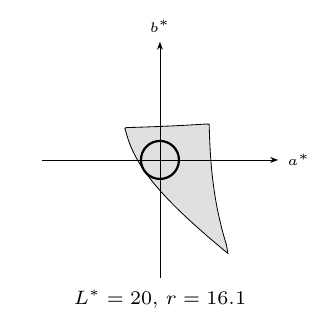
\begin{tikzpicture}[x=0.15mm, y=0.15mm, baseline=(label.base)]
    \useasboundingbox (-112,-125) rectangle (122,112);
    \draw[-{Stealth[length=1mm]}, line width=0.3pt] (-100,0) -- (100,0) node[right, font=\tiny] {$a^*$};
    \draw[-{Stealth[length=1mm]}, line width=0.3pt] (0,-100) -- (0,100) node[above, font=\tiny] {$b^*$};
    \fill[fill opacity=0.12] (43.08,0) -- (42.97,1.5) -- (42.86,3) -- (42.76,4.49) -- (42.67,6) -- (42.58,7.51) -- (42.49,9.03) -- (42.41,10.57) -- (42.33,12.14) -- (42.25,13.73) -- (42.18,15.35) -- (42.11,17.01) -- (42.05,18.72) -- (41.98,20.48) -- (41.92,22.29) -- (41.86,24.17) -- (41.79,26.12) -- (41.73,28.14) -- (41.65,30.26) -- (38.93,30.42) -- (36.03,30.23) -- (33.4,30.07) -- (30.99,29.93) -- (28.77,29.79) -- (26.72,29.68) -- (24.81,29.57) -- (23.03,29.47) -- (21.35,29.38) -- (19.76,29.3) -- (18.26,29.22) -- (16.83,29.14) -- (15.46,29.08) -- (14.15,29.01) -- (12.89,28.95) -- (11.67,28.89) -- (10.49,28.83) -- (9.35,28.78) -- (8.24,28.73) -- (7.15,28.68) -- (6.09,28.63) -- (5.04,28.59) -- (4.01,28.54) -- (3,28.5) -- (1.99,28.45) -- (0.99,28.41) -- (0,28.37) -- (-0.99,28.33) -- (-1.98,28.29) -- (-2.97,28.25) -- (-3.96,28.21) -- (-4.97,28.17) -- (-5.98,28.13) -- (-7,28.09) -- (-8.04,28.06) -- (-9.1,28.02) -- (-10.18,27.98) -- (-11.29,27.94) -- (-12.42,27.9) -- (-13.59,27.86) -- (-14.79,27.82) -- (-16.04,27.77) -- (-17.33,27.73) -- (-18.68,27.69) -- (-20.08,27.64) -- (-21.56,27.6) -- (-23.12,27.55) -- (-24.76,27.5) -- (-26.51,27.45) -- (-28.37,27.4) -- (-29.73,26.77) -- (-29.01,24.34) -- (-28.37,22.16) -- (-27.79,20.19) -- (-27.22,18.36) -- (-26.66,16.66) -- (-26.09,15.06) -- (-25.53,13.58) -- (-24.98,12.19) -- (-24.45,10.88) -- (-23.92,9.67) -- (-23.41,8.52) -- (-22.91,7.44) -- (-22.43,6.43) -- (-21.96,5.48) -- (-21.51,4.57) -- (-21.06,3.71) -- (-20.64,2.9) -- (-20.22,2.13) -- (-19.81,1.39) -- (-19.42,0.68) -- (-19.03,0) -- (-18.66,-0.65) -- (-18.29,-1.28) -- (-17.93,-1.88) -- (-17.58,-2.47) -- (-17.23,-3.04) -- (-16.89,-3.59) -- (-16.55,-4.13) -- (-16.22,-4.65) -- (-15.9,-5.17) -- (-15.57,-5.67) -- (-15.25,-6.16) -- (-14.93,-6.65) -- (-14.61,-7.13) -- (-14.29,-7.6) -- (-13.98,-8.07) -- (-13.66,-8.54) -- (-13.34,-9) -- (-13.02,-9.46) -- (-12.7,-9.92) -- (-12.37,-10.38) -- (-12.04,-10.84) -- (-11.71,-11.31) -- (-11.37,-11.78) -- (-11.03,-12.25) -- (-10.68,-12.72) -- (-10.32,-13.21) -- (-9.95,-13.7) -- (-9.58,-14.2) -- (-9.19,-14.71) -- (-8.79,-15.23) -- (-8.38,-15.76) -- (-7.95,-16.31) -- (-7.51,-16.87) -- (-7.05,-17.46) -- (-6.57,-18.06) -- (-6.07,-18.68) -- (-5.54,-19.33) -- (-4.99,-20.01) -- (-4.4,-20.72) -- (-3.78,-21.46) -- (-3.13,-22.24) -- (-2.42,-23.07) -- (-1.67,-23.94) -- (-0.87,-24.86) -- (0,-25.85) -- (0.94,-26.91) -- (1.96,-28.04) -- (3.08,-29.27) -- (4.3,-30.59) -- (5.65,-32.03) -- (7.14,-33.61) -- (8.81,-35.33) -- (10.68,-37.24) -- (12.79,-39.36) -- (15.19,-41.73) -- (17.94,-44.39) -- (21.11,-47.41) -- (24.8,-50.85) -- (29.14,-54.81) -- (34.31,-59.42) -- (40.52,-64.85) -- (48.1,-71.31) -- (57.5,-79.15) -- (56.34,-72.11) -- (54.08,-64.45) -- (52.4,-58.19) -- (51.09,-52.9) -- (50.03,-48.31) -- (49.16,-44.26) -- (48.43,-40.64) -- (47.8,-37.35) -- (47.27,-34.34) -- (46.8,-31.56) -- (46.38,-28.98) -- (46.01,-26.56) -- (45.68,-24.29) -- (45.38,-22.13) -- (45.11,-20.08) -- (44.86,-18.13) -- (44.64,-16.25) -- (44.43,-14.44) -- (44.23,-12.68) -- (44.06,-10.98) -- (43.89,-9.33) -- (43.73,-7.71) -- (43.59,-6.13) -- (43.45,-4.57) -- (43.32,-3.03) -- (43.2,-1.51) -- cycle;
    \draw[line width=0.3pt] (43.08,0) -- (42.97,1.5) -- (42.86,3) -- (42.76,4.49) -- (42.67,6) -- (42.58,7.51) -- (42.49,9.03) -- (42.41,10.57) -- (42.33,12.14) -- (42.25,13.73) -- (42.18,15.35) -- (42.11,17.01) -- (42.05,18.72) -- (41.98,20.48) -- (41.92,22.29) -- (41.86,24.17) -- (41.79,26.12) -- (41.73,28.14) -- (41.65,30.26) -- (38.93,30.42) -- (36.03,30.23) -- (33.4,30.07) -- (30.99,29.93) -- (28.77,29.79) -- (26.72,29.68) -- (24.81,29.57) -- (23.03,29.47) -- (21.35,29.38) -- (19.76,29.3) -- (18.26,29.22) -- (16.83,29.14) -- (15.46,29.08) -- (14.15,29.01) -- (12.89,28.95) -- (11.67,28.89) -- (10.49,28.83) -- (9.35,28.78) -- (8.24,28.73) -- (7.15,28.68) -- (6.09,28.63) -- (5.04,28.59) -- (4.01,28.54) -- (3,28.5) -- (1.99,28.45) -- (0.99,28.41) -- (0,28.37) -- (-0.99,28.33) -- (-1.98,28.29) -- (-2.97,28.25) -- (-3.96,28.21) -- (-4.97,28.17) -- (-5.98,28.13) -- (-7,28.09) -- (-8.04,28.06) -- (-9.1,28.02) -- (-10.18,27.98) -- (-11.29,27.94) -- (-12.42,27.9) -- (-13.59,27.86) -- (-14.79,27.82) -- (-16.04,27.77) -- (-17.33,27.73) -- (-18.68,27.69) -- (-20.08,27.64) -- (-21.56,27.6) -- (-23.12,27.55) -- (-24.76,27.5) -- (-26.51,27.45) -- (-28.37,27.4) -- (-29.73,26.77) -- (-29.01,24.34) -- (-28.37,22.16) -- (-27.79,20.19) -- (-27.22,18.36) -- (-26.66,16.66) -- (-26.09,15.06) -- (-25.53,13.58) -- (-24.98,12.19) -- (-24.45,10.88) -- (-23.92,9.67) -- (-23.41,8.52) -- (-22.91,7.44) -- (-22.43,6.43) -- (-21.96,5.48) -- (-21.51,4.57) -- (-21.06,3.71) -- (-20.64,2.9) -- (-20.22,2.13) -- (-19.81,1.39) -- (-19.42,0.68) -- (-19.03,0) -- (-18.66,-0.65) -- (-18.29,-1.28) -- (-17.93,-1.88) -- (-17.58,-2.47) -- (-17.23,-3.04) -- (-16.89,-3.59) -- (-16.55,-4.13) -- (-16.22,-4.65) -- (-15.9,-5.17) -- (-15.57,-5.67) -- (-15.25,-6.16) -- (-14.93,-6.65) -- (-14.61,-7.13) -- (-14.29,-7.6) -- (-13.98,-8.07) -- (-13.66,-8.54) -- (-13.34,-9) -- (-13.02,-9.46) -- (-12.7,-9.92) -- (-12.37,-10.38) -- (-12.04,-10.84) -- (-11.71,-11.31) -- (-11.37,-11.78) -- (-11.03,-12.25) -- (-10.68,-12.72) -- (-10.32,-13.21) -- (-9.95,-13.7) -- (-9.58,-14.2) -- (-9.19,-14.71) -- (-8.79,-15.23) -- (-8.38,-15.76) -- (-7.95,-16.31) -- (-7.51,-16.87) -- (-7.05,-17.46) -- (-6.57,-18.06) -- (-6.07,-18.68) -- (-5.54,-19.33) -- (-4.99,-20.01) -- (-4.4,-20.72) -- (-3.78,-21.46) -- (-3.13,-22.24) -- (-2.42,-23.07) -- (-1.67,-23.94) -- (-0.87,-24.86) -- (0,-25.85) -- (0.94,-26.91) -- (1.96,-28.04) -- (3.08,-29.27) -- (4.3,-30.59) -- (5.65,-32.03) -- (7.14,-33.61) -- (8.81,-35.33) -- (10.68,-37.24) -- (12.79,-39.36) -- (15.19,-41.73) -- (17.94,-44.39) -- (21.11,-47.41) -- (24.8,-50.85) -- (29.14,-54.81) -- (34.31,-59.42) -- (40.52,-64.85) -- (48.1,-71.31) -- (57.5,-79.15) -- (56.34,-72.11) -- (54.08,-64.45) -- (52.4,-58.19) -- (51.09,-52.9) -- (50.03,-48.31) -- (49.16,-44.26) -- (48.43,-40.64) -- (47.8,-37.35) -- (47.27,-34.34) -- (46.8,-31.56) -- (46.38,-28.98) -- (46.01,-26.56) -- (45.68,-24.29) -- (45.38,-22.13) -- (45.11,-20.08) -- (44.86,-18.13) -- (44.64,-16.25) -- (44.43,-14.44) -- (44.23,-12.68) -- (44.06,-10.98) -- (43.89,-9.33) -- (43.73,-7.71) -- (43.59,-6.13) -- (43.45,-4.57) -- (43.32,-3.03) -- (43.2,-1.51) -- cycle;
    \draw[thick] (0,0) circle[radius=16.09];
    \node[font=\scriptsize] (label) at (0,-118) {$L^* = 20$, $r = 16.1$};
  \end{tikzpicture}%
  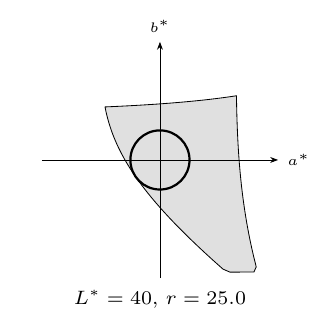
\begin{tikzpicture}[x=0.15mm, y=0.15mm, baseline=(label.base)]
    \useasboundingbox (-112,-125) rectangle (122,112);
    \draw[-{Stealth[length=1mm]}, line width=0.3pt] (-100,0) -- (100,0) node[right, font=\tiny] {$a^*$};
    \draw[-{Stealth[length=1mm]}, line width=0.3pt] (0,-100) -- (0,100) node[above, font=\tiny] {$b^*$};
    \fill[fill opacity=0.12] (67.01,0) -- (66.84,2.33) -- (66.68,4.66) -- (66.52,6.99) -- (66.37,9.33) -- (66.23,11.68) -- (66.1,14.05) -- (65.97,16.45) -- (65.85,18.88) -- (65.73,21.36) -- (65.62,23.88) -- (65.51,26.47) -- (65.41,29.12) -- (65.31,31.85) -- (65.22,34.68) -- (65.13,37.6) -- (65.05,40.65) -- (64.97,43.82) -- (64.9,47.15) -- (64.84,50.65) -- (64.77,54.35) -- (59.49,53.56) -- (54.79,52.91) -- (50.55,52.35) -- (46.7,51.87) -- (43.17,51.44) -- (39.9,51.07) -- (36.86,50.73) -- (34.02,50.43) -- (31.34,50.15) -- (28.81,49.9) -- (26.41,49.67) -- (24.12,49.45) -- (21.93,49.25) -- (19.82,49.06) -- (17.79,48.88) -- (15.83,48.71) -- (13.92,48.55) -- (12.07,48.4) -- (10.26,48.25) -- (8.48,48.11) -- (6.74,47.98) -- (5.03,47.85) -- (3.34,47.72) -- (1.66,47.6) -- (0,47.48) -- (-1.65,47.36) -- (-3.3,47.25) -- (-4.95,47.14) -- (-6.61,47.03) -- (-8.27,46.92) -- (-9.95,46.81) -- (-11.64,46.7) -- (-13.36,46.6) -- (-15.11,46.49) -- (-16.88,46.38) -- (-18.7,46.28) -- (-20.56,46.17) -- (-22.47,46.07) -- (-24.44,45.96) -- (-26.47,45.85) -- (-28.58,45.74) -- (-30.78,45.63) -- (-33.07,45.51) -- (-35.47,45.4) -- (-37.99,45.28) -- (-40.66,45.16) -- (-43.49,45.03) -- (-46.5,44.9) -- (-45.76,41.2) -- (-44.94,37.71) -- (-44.1,34.45) -- (-43.23,31.41) -- (-42.35,28.56) -- (-41.47,25.91) -- (-40.59,23.43) -- (-39.72,21.12) -- (-38.87,18.96) -- (-38.03,16.93) -- (-37.21,15.03) -- (-36.42,13.25) -- (-35.64,11.58) -- (-34.89,10) -- (-34.16,8.52) -- (-33.45,7.11) -- (-32.77,5.78) -- (-32.1,4.51) -- (-31.45,3.31) -- (-30.82,2.16) -- (-30.21,1.05) -- (-29.61,0) -- (-29.02,-1.01) -- (-28.45,-1.99) -- (-27.89,-2.93) -- (-27.34,-3.84) -- (-26.8,-4.73) -- (-26.27,-5.58) -- (-25.75,-6.42) -- (-25.24,-7.24) -- (-24.73,-8.03) -- (-24.22,-8.82) -- (-23.72,-9.58) -- (-23.23,-10.34) -- (-22.73,-11.09) -- (-22.24,-11.82) -- (-21.74,-12.55) -- (-21.25,-13.28) -- (-20.75,-14) -- (-20.25,-14.72) -- (-19.75,-15.43) -- (-19.25,-16.15) -- (-18.73,-16.87) -- (-18.22,-17.59) -- (-17.69,-18.32) -- (-17.15,-19.05) -- (-16.61,-19.79) -- (-16.05,-20.55) -- (-15.48,-21.31) -- (-14.9,-22.09) -- (-14.3,-22.88) -- (-13.68,-23.69) -- (-13.04,-24.52) -- (-12.37,-25.37) -- (-11.69,-26.25) -- (-10.97,-27.15) -- (-10.22,-28.09) -- (-9.44,-29.06) -- (-8.62,-30.07) -- (-7.76,-31.13) -- (-6.85,-32.23) -- (-5.89,-33.38) -- (-4.86,-34.6) -- (-3.77,-35.88) -- (-2.6,-37.24) -- (-1.35,-38.68) -- (0,-40.22) -- (1.46,-41.86) -- (3.05,-43.62) -- (4.79,-45.53) -- (6.69,-47.59) -- (8.79,-49.83) -- (11.11,-52.28) -- (13.7,-54.97) -- (16.61,-57.93) -- (19.89,-61.23) -- (23.63,-64.91) -- (27.9,-69.05) -- (32.83,-73.74) -- (38.58,-79.1) -- (45.33,-85.26) -- (53.37,-92.43) -- (59.37,-95.01) -- (64.06,-94.97) -- (68.97,-94.93) -- (74.14,-94.89) -- (79.59,-94.85) -- (81.51,-90.52) -- (79.47,-82.29) -- (77.82,-75.15) -- (76.47,-68.85) -- (75.33,-63.21) -- (74.36,-58.1) -- (73.52,-53.42) -- (72.79,-49.1) -- (72.15,-45.08) -- (71.57,-41.32) -- (71.06,-37.78) -- (70.59,-34.43) -- (70.17,-31.24) -- (69.79,-28.2) -- (69.43,-25.27) -- (69.11,-22.46) -- (68.81,-19.73) -- (68.53,-17.09) -- (68.27,-14.51) -- (68.03,-12) -- (67.8,-9.53) -- (67.59,-7.1) -- (67.38,-4.71) -- (67.19,-2.35) -- cycle;
    \draw[line width=0.3pt] (67.01,0) -- (66.84,2.33) -- (66.68,4.66) -- (66.52,6.99) -- (66.37,9.33) -- (66.23,11.68) -- (66.1,14.05) -- (65.97,16.45) -- (65.85,18.88) -- (65.73,21.36) -- (65.62,23.88) -- (65.51,26.47) -- (65.41,29.12) -- (65.31,31.85) -- (65.22,34.68) -- (65.13,37.6) -- (65.05,40.65) -- (64.97,43.82) -- (64.9,47.15) -- (64.84,50.65) -- (64.77,54.35) -- (59.49,53.56) -- (54.79,52.91) -- (50.55,52.35) -- (46.7,51.87) -- (43.17,51.44) -- (39.9,51.07) -- (36.86,50.73) -- (34.02,50.43) -- (31.34,50.15) -- (28.81,49.9) -- (26.41,49.67) -- (24.12,49.45) -- (21.93,49.25) -- (19.82,49.06) -- (17.79,48.88) -- (15.83,48.71) -- (13.92,48.55) -- (12.07,48.4) -- (10.26,48.25) -- (8.48,48.11) -- (6.74,47.98) -- (5.03,47.85) -- (3.34,47.72) -- (1.66,47.6) -- (0,47.48) -- (-1.65,47.36) -- (-3.3,47.25) -- (-4.95,47.14) -- (-6.61,47.03) -- (-8.27,46.92) -- (-9.95,46.81) -- (-11.64,46.7) -- (-13.36,46.6) -- (-15.11,46.49) -- (-16.88,46.38) -- (-18.7,46.28) -- (-20.56,46.17) -- (-22.47,46.07) -- (-24.44,45.96) -- (-26.47,45.85) -- (-28.58,45.74) -- (-30.78,45.63) -- (-33.07,45.51) -- (-35.47,45.4) -- (-37.99,45.28) -- (-40.66,45.16) -- (-43.49,45.03) -- (-46.5,44.9) -- (-45.76,41.2) -- (-44.94,37.71) -- (-44.1,34.45) -- (-43.23,31.41) -- (-42.35,28.56) -- (-41.47,25.91) -- (-40.59,23.43) -- (-39.72,21.12) -- (-38.87,18.96) -- (-38.03,16.93) -- (-37.21,15.03) -- (-36.42,13.25) -- (-35.64,11.58) -- (-34.89,10) -- (-34.16,8.52) -- (-33.45,7.11) -- (-32.77,5.78) -- (-32.1,4.51) -- (-31.45,3.31) -- (-30.82,2.16) -- (-30.21,1.05) -- (-29.61,0) -- (-29.02,-1.01) -- (-28.45,-1.99) -- (-27.89,-2.93) -- (-27.34,-3.84) -- (-26.8,-4.73) -- (-26.27,-5.58) -- (-25.75,-6.42) -- (-25.24,-7.24) -- (-24.73,-8.03) -- (-24.22,-8.82) -- (-23.72,-9.58) -- (-23.23,-10.34) -- (-22.73,-11.09) -- (-22.24,-11.82) -- (-21.74,-12.55) -- (-21.25,-13.28) -- (-20.75,-14) -- (-20.25,-14.72) -- (-19.75,-15.43) -- (-19.25,-16.15) -- (-18.73,-16.87) -- (-18.22,-17.59) -- (-17.69,-18.32) -- (-17.15,-19.05) -- (-16.61,-19.79) -- (-16.05,-20.55) -- (-15.48,-21.31) -- (-14.9,-22.09) -- (-14.3,-22.88) -- (-13.68,-23.69) -- (-13.04,-24.52) -- (-12.37,-25.37) -- (-11.69,-26.25) -- (-10.97,-27.15) -- (-10.22,-28.09) -- (-9.44,-29.06) -- (-8.62,-30.07) -- (-7.76,-31.13) -- (-6.85,-32.23) -- (-5.89,-33.38) -- (-4.86,-34.6) -- (-3.77,-35.88) -- (-2.6,-37.24) -- (-1.35,-38.68) -- (0,-40.22) -- (1.46,-41.86) -- (3.05,-43.62) -- (4.79,-45.53) -- (6.69,-47.59) -- (8.79,-49.83) -- (11.11,-52.28) -- (13.7,-54.97) -- (16.61,-57.93) -- (19.89,-61.23) -- (23.63,-64.91) -- (27.9,-69.05) -- (32.83,-73.74) -- (38.58,-79.1) -- (45.33,-85.26) -- (53.37,-92.43) -- (59.37,-95.01) -- (64.06,-94.97) -- (68.97,-94.93) -- (74.14,-94.89) -- (79.59,-94.85) -- (81.51,-90.52) -- (79.47,-82.29) -- (77.82,-75.15) -- (76.47,-68.85) -- (75.33,-63.21) -- (74.36,-58.1) -- (73.52,-53.42) -- (72.79,-49.1) -- (72.15,-45.08) -- (71.57,-41.32) -- (71.06,-37.78) -- (70.59,-34.43) -- (70.17,-31.24) -- (69.79,-28.2) -- (69.43,-25.27) -- (69.11,-22.46) -- (68.81,-19.73) -- (68.53,-17.09) -- (68.27,-14.51) -- (68.03,-12) -- (67.8,-9.53) -- (67.59,-7.1) -- (67.38,-4.71) -- (67.19,-2.35) -- cycle;
    \draw[thick] (0,0) circle[radius=25.03];
    \node[font=\scriptsize] (label) at (0,-118) {$L^* = 40$, $r = 25.0$};
  \end{tikzpicture}%
  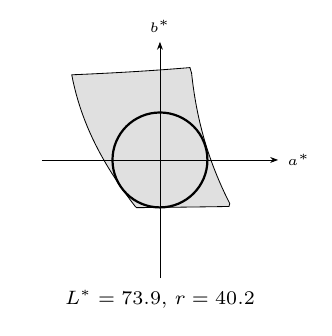
\begin{tikzpicture}[x=0.15mm, y=0.15mm, baseline=(label.base)]
    \useasboundingbox (-112,-125) rectangle (122,112);
    \draw[-{Stealth[length=1mm]}, line width=0.3pt] (-100,0) -- (100,0) node[right, font=\tiny] {$a^*$};
    \draw[-{Stealth[length=1mm]}, line width=0.3pt] (0,-100) -- (0,100) node[above, font=\tiny] {$b^*$};
    \fill[fill opacity=0.12] (43.15,0) -- (42.62,1.49) -- (42.11,2.94) -- (41.62,4.37) -- (41.15,5.78) -- (40.69,7.17) -- (40.24,8.55) -- (39.8,9.92) -- (39.37,11.29) -- (38.95,12.66) -- (38.53,14.02) -- (38.12,15.4) -- (37.71,16.79) -- (37.31,18.2) -- (36.9,19.62) -- (36.5,21.07) -- (36.1,22.56) -- (35.69,24.08) -- (35.29,25.64) -- (34.88,27.25) -- (34.46,28.92) -- (34.04,30.65) -- (33.61,32.46) -- (33.18,34.35) -- (32.73,36.35) -- (32.27,38.46) -- (31.81,40.71) -- (31.32,43.11) -- (30.83,45.7) -- (30.31,48.51) -- (29.78,51.58) -- (29.22,54.96) -- (28.65,58.73) -- (28.04,62.99) -- (27.42,67.87) -- (26.77,73.55) -- (25.41,78.21) -- (22.35,77.95) -- (19.37,77.71) -- (16.47,77.47) -- (13.62,77.25) -- (10.83,77.03) -- (8.07,76.82) -- (5.36,76.62) -- (2.67,76.42) -- (0,76.23) -- (-2.66,76.04) -- (-5.3,75.86) -- (-7.95,75.68) -- (-10.61,75.5) -- (-13.28,75.33) -- (-15.97,75.16) -- (-18.7,74.98) -- (-21.45,74.81) -- (-24.25,74.64) -- (-27.11,74.47) -- (-30.02,74.3) -- (-33.01,74.13) -- (-36.07,73.96) -- (-39.23,73.79) -- (-42.5,73.61) -- (-45.89,73.44) -- (-49.41,73.26) -- (-53.09,73.08) -- (-56.95,72.89) -- (-61,72.7) -- (-65.28,72.5) -- (-69.82,72.3) -- (-74.66,72.1) -- (-73.47,66.15) -- (-72.16,60.55) -- (-70.8,55.32) -- (-69.41,50.43) -- (-67.99,45.86) -- (-66.58,41.6) -- (-65.17,37.62) -- (-63.77,33.91) -- (-62.4,30.44) -- (-61.06,27.18) -- (-59.75,24.14) -- (-58.47,21.28) -- (-57.23,18.59) -- (-56.02,16.06) -- (-54.85,13.68) -- (-53.71,11.42) -- (-52.61,9.28) -- (-51.54,7.24) -- (-50.5,5.31) -- (-49.48,3.46) -- (-48.5,1.69) -- (-47.54,0) -- (-46.6,-1.63) -- (-45.68,-3.19) -- (-44.78,-4.71) -- (-43.9,-6.17) -- (-43.04,-7.59) -- (-42.19,-8.97) -- (-41.35,-10.31) -- (-40.52,-11.62) -- (-39.7,-12.9) -- (-38.89,-14.16) -- (-38.09,-15.39) -- (-37.29,-16.6) -- (-36.49,-17.8) -- (-35.7,-18.98) -- (-34.91,-20.15) -- (-34.12,-21.32) -- (-33.32,-22.47) -- (-32.52,-23.63) -- (-31.71,-24.78) -- (-30.9,-25.93) -- (-30.08,-27.08) -- (-29.25,-28.24) -- (-28.4,-29.41) -- (-27.54,-30.59) -- (-26.67,-31.78) -- (-25.77,-32.99) -- (-24.86,-34.21) -- (-23.92,-35.46) -- (-22.95,-36.73) -- (-21.96,-38.03) -- (-20.93,-39.37) -- (-19.71,-40.4) -- (-17.98,-40.39) -- (-16.31,-40.37) -- (-14.69,-40.35) -- (-13.11,-40.33) -- (-11.56,-40.32) -- (-10.05,-40.3) -- (-8.56,-40.28) -- (-7.1,-40.27) -- (-5.66,-40.25) -- (-4.23,-40.24) -- (-2.81,-40.22) -- (-1.4,-40.2) -- (0,-40.19) -- (1.4,-40.17) -- (2.81,-40.16) -- (4.22,-40.14) -- (5.64,-40.12) -- (7.07,-40.1) -- (8.52,-40.09) -- (9.99,-40.07) -- (11.48,-40.05) -- (13.01,-40.03) -- (14.56,-40.01) -- (16.16,-39.99) -- (17.8,-39.97) -- (19.49,-39.95) -- (21.23,-39.93) -- (23.04,-39.9) -- (24.92,-39.88) -- (26.88,-39.85) -- (28.94,-39.83) -- (31.09,-39.8) -- (33.37,-39.77) -- (35.78,-39.73) -- (38.33,-39.7) -- (41.07,-39.66) -- (44,-39.62) -- (47.16,-39.57) -- (50.58,-39.52) -- (54.32,-39.46) -- (58.41,-39.4) -- (59.11,-36.94) -- (57.14,-32.99) -- (55.43,-29.47) -- (53.94,-26.31) -- (52.62,-23.43) -- (51.44,-20.78) -- (50.37,-18.33) -- (49.39,-16.05) -- (48.5,-13.91) -- (47.67,-11.89) -- (46.9,-9.97) -- (46.18,-8.14) -- (45.51,-6.4) -- (44.87,-4.72) -- (44.27,-3.1) -- (43.69,-1.53) -- cycle;
    \draw[line width=0.3pt] (43.15,0) -- (42.62,1.49) -- (42.11,2.94) -- (41.62,4.37) -- (41.15,5.78) -- (40.69,7.17) -- (40.24,8.55) -- (39.8,9.92) -- (39.37,11.29) -- (38.95,12.66) -- (38.53,14.02) -- (38.12,15.4) -- (37.71,16.79) -- (37.31,18.2) -- (36.9,19.62) -- (36.5,21.07) -- (36.1,22.56) -- (35.69,24.08) -- (35.29,25.64) -- (34.88,27.25) -- (34.46,28.92) -- (34.04,30.65) -- (33.61,32.46) -- (33.18,34.35) -- (32.73,36.35) -- (32.27,38.46) -- (31.81,40.71) -- (31.32,43.11) -- (30.83,45.7) -- (30.31,48.51) -- (29.78,51.58) -- (29.22,54.96) -- (28.65,58.73) -- (28.04,62.99) -- (27.42,67.87) -- (26.77,73.55) -- (25.41,78.21) -- (22.35,77.95) -- (19.37,77.71) -- (16.47,77.47) -- (13.62,77.25) -- (10.83,77.03) -- (8.07,76.82) -- (5.36,76.62) -- (2.67,76.42) -- (0,76.23) -- (-2.66,76.04) -- (-5.3,75.86) -- (-7.95,75.68) -- (-10.61,75.5) -- (-13.28,75.33) -- (-15.97,75.16) -- (-18.7,74.98) -- (-21.45,74.81) -- (-24.25,74.64) -- (-27.11,74.47) -- (-30.02,74.3) -- (-33.01,74.13) -- (-36.07,73.96) -- (-39.23,73.79) -- (-42.5,73.61) -- (-45.89,73.44) -- (-49.41,73.26) -- (-53.09,73.08) -- (-56.95,72.89) -- (-61,72.7) -- (-65.28,72.5) -- (-69.82,72.3) -- (-74.66,72.1) -- (-73.47,66.15) -- (-72.16,60.55) -- (-70.8,55.32) -- (-69.41,50.43) -- (-67.99,45.86) -- (-66.58,41.6) -- (-65.17,37.62) -- (-63.77,33.91) -- (-62.4,30.44) -- (-61.06,27.18) -- (-59.75,24.14) -- (-58.47,21.28) -- (-57.23,18.59) -- (-56.02,16.06) -- (-54.85,13.68) -- (-53.71,11.42) -- (-52.61,9.28) -- (-51.54,7.24) -- (-50.5,5.31) -- (-49.48,3.46) -- (-48.5,1.69) -- (-47.54,0) -- (-46.6,-1.63) -- (-45.68,-3.19) -- (-44.78,-4.71) -- (-43.9,-6.17) -- (-43.04,-7.59) -- (-42.19,-8.97) -- (-41.35,-10.31) -- (-40.52,-11.62) -- (-39.7,-12.9) -- (-38.89,-14.16) -- (-38.09,-15.39) -- (-37.29,-16.6) -- (-36.49,-17.8) -- (-35.7,-18.98) -- (-34.91,-20.15) -- (-34.12,-21.32) -- (-33.32,-22.47) -- (-32.52,-23.63) -- (-31.71,-24.78) -- (-30.9,-25.93) -- (-30.08,-27.08) -- (-29.25,-28.24) -- (-28.4,-29.41) -- (-27.54,-30.59) -- (-26.67,-31.78) -- (-25.77,-32.99) -- (-24.86,-34.21) -- (-23.92,-35.46) -- (-22.95,-36.73) -- (-21.96,-38.03) -- (-20.93,-39.37) -- (-19.71,-40.4) -- (-17.98,-40.39) -- (-16.31,-40.37) -- (-14.69,-40.35) -- (-13.11,-40.33) -- (-11.56,-40.32) -- (-10.05,-40.3) -- (-8.56,-40.28) -- (-7.1,-40.27) -- (-5.66,-40.25) -- (-4.23,-40.24) -- (-2.81,-40.22) -- (-1.4,-40.2) -- (0,-40.19) -- (1.4,-40.17) -- (2.81,-40.16) -- (4.22,-40.14) -- (5.64,-40.12) -- (7.07,-40.1) -- (8.52,-40.09) -- (9.99,-40.07) -- (11.48,-40.05) -- (13.01,-40.03) -- (14.56,-40.01) -- (16.16,-39.99) -- (17.8,-39.97) -- (19.49,-39.95) -- (21.23,-39.93) -- (23.04,-39.9) -- (24.92,-39.88) -- (26.88,-39.85) -- (28.94,-39.83) -- (31.09,-39.8) -- (33.37,-39.77) -- (35.78,-39.73) -- (38.33,-39.7) -- (41.07,-39.66) -- (44,-39.62) -- (47.16,-39.57) -- (50.58,-39.52) -- (54.32,-39.46) -- (58.41,-39.4) -- (59.11,-36.94) -- (57.14,-32.99) -- (55.43,-29.47) -- (53.94,-26.31) -- (52.62,-23.43) -- (51.44,-20.78) -- (50.37,-18.33) -- (49.39,-16.05) -- (48.5,-13.91) -- (47.67,-11.89) -- (46.9,-9.97) -- (46.18,-8.14) -- (45.51,-6.4) -- (44.87,-4.72) -- (44.27,-3.1) -- (43.69,-1.53) -- cycle;
    \draw[thick] (0,0) circle[radius=40.19];
    \node[font=\scriptsize] (label) at (0,-118) {$L^* = 73.9$, $r = 40.2$};
  \end{tikzpicture}%
  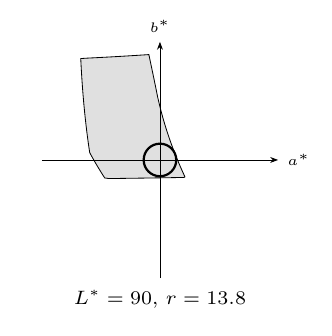
\begin{tikzpicture}[x=0.15mm, y=0.15mm, baseline=(label.base)]
    \useasboundingbox (-112,-125) rectangle (122,112);
    \draw[-{Stealth[length=1mm]}, line width=0.3pt] (-100,0) -- (100,0) node[right, font=\tiny] {$a^*$};
    \draw[-{Stealth[length=1mm]}, line width=0.3pt] (0,-100) -- (0,100) node[above, font=\tiny] {$b^*$};
    \fill[fill opacity=0.12] (14.87,0) -- (14.66,0.51) -- (14.45,1.01) -- (14.25,1.5) -- (14.06,1.98) -- (13.87,2.45) -- (13.68,2.91) -- (13.5,3.37) -- (13.32,3.82) -- (13.14,4.27) -- (12.96,4.72) -- (12.78,5.16) -- (12.61,5.61) -- (12.43,6.06) -- (12.26,6.52) -- (12.08,6.97) -- (11.9,7.44) -- (11.72,7.9) -- (11.54,8.38) -- (11.35,8.87) -- (11.16,9.37) -- (10.97,9.88) -- (10.77,10.4) -- (10.57,10.95) -- (10.36,11.51) -- (10.15,12.09) -- (9.92,12.7) -- (9.69,13.34) -- (9.45,14.01) -- (9.19,14.71) -- (8.93,15.46) -- (8.65,16.26) -- (8.35,17.11) -- (8.03,18.03) -- (7.69,19.02) -- (7.32,20.11) -- (6.92,21.3) -- (6.48,22.61) -- (6,24.08) -- (5.47,25.74) -- (4.87,27.64) -- (4.2,29.85) -- (3.41,32.48) -- (2.49,35.67) -- (1.39,39.7) -- (0,45.04) -- (-1.84,52.82) -- (-4.67,66.75) -- (-9.38,89.22) -- (-12.51,89.01) -- (-15.66,88.81) -- (-18.83,88.6) -- (-22.04,88.4) -- (-25.29,88.2) -- (-28.59,88) -- (-31.96,87.8) -- (-35.39,87.6) -- (-38.91,87.4) -- (-42.53,87.2) -- (-46.25,86.99) -- (-50.11,86.79) -- (-54.1,86.58) -- (-58.25,86.37) -- (-62.59,86.15) -- (-67.07,85.84) -- (-66.75,79.55) -- (-66.42,73.77) -- (-66.09,68.44) -- (-65.75,63.49) -- (-65.41,58.89) -- (-65.07,54.6) -- (-64.73,50.57) -- (-64.39,46.78) -- (-64.05,43.2) -- (-63.71,39.81) -- (-63.38,36.59) -- (-63.05,33.52) -- (-62.72,30.59) -- (-62.39,27.78) -- (-62.07,25.08) -- (-61.74,22.47) -- (-61.42,19.96) -- (-61.1,17.52) -- (-60.78,15.15) -- (-60.46,12.85) -- (-60.14,10.6) -- (-59.81,8.41) -- (-59.49,6.25) -- (-58.34,4.08) -- (-57.17,2) -- (-56.04,0) -- (-54.93,-1.92) -- (-53.85,-3.77) -- (-52.79,-5.55) -- (-51.76,-7.27) -- (-50.74,-8.95) -- (-49.73,-10.57) -- (-48.75,-12.15) -- (-47.77,-13.7) -- (-46.81,-15.21) -- (-43.3,-15.76) -- (-38.87,-15.7) -- (-35.16,-15.65) -- (-32.01,-15.61) -- (-29.29,-15.57) -- (-26.92,-15.54) -- (-24.83,-15.51) -- (-22.96,-15.49) -- (-21.28,-15.46) -- (-19.76,-15.44) -- (-18.38,-15.42) -- (-17.11,-15.4) -- (-15.93,-15.39) -- (-14.84,-15.37) -- (-13.83,-15.36) -- (-12.87,-15.34) -- (-11.98,-15.33) -- (-11.13,-15.32) -- (-10.32,-15.3) -- (-9.56,-15.29) -- (-8.82,-15.28) -- (-8.12,-15.27) -- (-7.44,-15.26) -- (-6.79,-15.25) -- (-6.16,-15.24) -- (-5.54,-15.23) -- (-4.95,-15.22) -- (-4.36,-15.21) -- (-3.79,-15.2) -- (-3.23,-15.2) -- (-2.68,-15.19) -- (-2.13,-15.18) -- (-1.59,-15.17) -- (-1.06,-15.16) -- (-0.53,-15.15) -- (0,-15.15) -- (0.53,-15.14) -- (1.06,-15.13) -- (1.59,-15.12) -- (2.12,-15.11) -- (2.66,-15.1) -- (3.21,-15.09) -- (3.76,-15.09) -- (4.32,-15.08) -- (4.9,-15.07) -- (5.48,-15.06) -- (6.08,-15.05) -- (6.7,-15.04) -- (7.33,-15.03) -- (7.99,-15.02) -- (8.66,-15.01) -- (9.37,-15) -- (10.11,-14.98) -- (10.88,-14.97) -- (11.69,-14.96) -- (12.54,-14.94) -- (13.44,-14.93) -- (14.4,-14.91) -- (15.42,-14.9) -- (16.52,-14.88) -- (17.71,-14.86) -- (18.99,-14.83) -- (20.39,-14.81) -- (21.15,-14.27) -- (20.46,-12.79) -- (19.86,-11.46) -- (19.31,-10.27) -- (18.82,-9.18) -- (18.38,-8.18) -- (17.97,-7.26) -- (17.59,-6.4) -- (17.24,-5.6) -- (16.92,-4.85) -- (16.61,-4.14) -- (16.32,-3.47) -- (16.05,-2.83) -- (15.79,-2.22) -- (15.55,-1.63) -- (15.31,-1.07) -- (15.09,-0.53) -- cycle;
    \draw[line width=0.3pt] (14.87,0) -- (14.66,0.51) -- (14.45,1.01) -- (14.25,1.5) -- (14.06,1.98) -- (13.87,2.45) -- (13.68,2.91) -- (13.5,3.37) -- (13.32,3.82) -- (13.14,4.27) -- (12.96,4.72) -- (12.78,5.16) -- (12.61,5.61) -- (12.43,6.06) -- (12.26,6.52) -- (12.08,6.97) -- (11.9,7.44) -- (11.72,7.9) -- (11.54,8.38) -- (11.35,8.87) -- (11.16,9.37) -- (10.97,9.88) -- (10.77,10.4) -- (10.57,10.95) -- (10.36,11.51) -- (10.15,12.09) -- (9.92,12.7) -- (9.69,13.34) -- (9.45,14.01) -- (9.19,14.71) -- (8.93,15.46) -- (8.65,16.26) -- (8.35,17.11) -- (8.03,18.03) -- (7.69,19.02) -- (7.32,20.11) -- (6.92,21.3) -- (6.48,22.61) -- (6,24.08) -- (5.47,25.74) -- (4.87,27.64) -- (4.2,29.85) -- (3.41,32.48) -- (2.49,35.67) -- (1.39,39.7) -- (0,45.04) -- (-1.84,52.82) -- (-4.67,66.75) -- (-9.38,89.22) -- (-12.51,89.01) -- (-15.66,88.81) -- (-18.83,88.6) -- (-22.04,88.4) -- (-25.29,88.2) -- (-28.59,88) -- (-31.96,87.8) -- (-35.39,87.6) -- (-38.91,87.4) -- (-42.53,87.2) -- (-46.25,86.99) -- (-50.11,86.79) -- (-54.1,86.58) -- (-58.25,86.37) -- (-62.59,86.15) -- (-67.07,85.84) -- (-66.75,79.55) -- (-66.42,73.77) -- (-66.09,68.44) -- (-65.75,63.49) -- (-65.41,58.89) -- (-65.07,54.6) -- (-64.73,50.57) -- (-64.39,46.78) -- (-64.05,43.2) -- (-63.71,39.81) -- (-63.38,36.59) -- (-63.05,33.52) -- (-62.72,30.59) -- (-62.39,27.78) -- (-62.07,25.08) -- (-61.74,22.47) -- (-61.42,19.96) -- (-61.1,17.52) -- (-60.78,15.15) -- (-60.46,12.85) -- (-60.14,10.6) -- (-59.81,8.41) -- (-59.49,6.25) -- (-58.34,4.08) -- (-57.17,2) -- (-56.04,0) -- (-54.93,-1.92) -- (-53.85,-3.77) -- (-52.79,-5.55) -- (-51.76,-7.27) -- (-50.74,-8.95) -- (-49.73,-10.57) -- (-48.75,-12.15) -- (-47.77,-13.7) -- (-46.81,-15.21) -- (-43.3,-15.76) -- (-38.87,-15.7) -- (-35.16,-15.65) -- (-32.01,-15.61) -- (-29.29,-15.57) -- (-26.92,-15.54) -- (-24.83,-15.51) -- (-22.96,-15.49) -- (-21.28,-15.46) -- (-19.76,-15.44) -- (-18.38,-15.42) -- (-17.11,-15.4) -- (-15.93,-15.39) -- (-14.84,-15.37) -- (-13.83,-15.36) -- (-12.87,-15.34) -- (-11.98,-15.33) -- (-11.13,-15.32) -- (-10.32,-15.3) -- (-9.56,-15.29) -- (-8.82,-15.28) -- (-8.12,-15.27) -- (-7.44,-15.26) -- (-6.79,-15.25) -- (-6.16,-15.24) -- (-5.54,-15.23) -- (-4.95,-15.22) -- (-4.36,-15.21) -- (-3.79,-15.2) -- (-3.23,-15.2) -- (-2.68,-15.19) -- (-2.13,-15.18) -- (-1.59,-15.17) -- (-1.06,-15.16) -- (-0.53,-15.15) -- (0,-15.15) -- (0.53,-15.14) -- (1.06,-15.13) -- (1.59,-15.12) -- (2.12,-15.11) -- (2.66,-15.1) -- (3.21,-15.09) -- (3.76,-15.09) -- (4.32,-15.08) -- (4.9,-15.07) -- (5.48,-15.06) -- (6.08,-15.05) -- (6.7,-15.04) -- (7.33,-15.03) -- (7.99,-15.02) -- (8.66,-15.01) -- (9.37,-15) -- (10.11,-14.98) -- (10.88,-14.97) -- (11.69,-14.96) -- (12.54,-14.94) -- (13.44,-14.93) -- (14.4,-14.91) -- (15.42,-14.9) -- (16.52,-14.88) -- (17.71,-14.86) -- (18.99,-14.83) -- (20.39,-14.81) -- (21.15,-14.27) -- (20.46,-12.79) -- (19.86,-11.46) -- (19.31,-10.27) -- (18.82,-9.18) -- (18.38,-8.18) -- (17.97,-7.26) -- (17.59,-6.4) -- (17.24,-5.6) -- (16.92,-4.85) -- (16.61,-4.14) -- (16.32,-3.47) -- (16.05,-2.83) -- (15.79,-2.22) -- (15.55,-1.63) -- (15.31,-1.07) -- (15.09,-0.53) -- cycle;
    \draw[thick] (0,0) circle[radius=13.79];
    \node[font=\scriptsize] (label) at (0,-118) {$L^* = 90$, $r = 13.8$};
  \end{tikzpicture}

  The gamut narrows toward black and white, and so does the 256-gon.
\end{slide}

\begin{slide}{The radius over lightness}
  \centering
  \begin{tikzpicture}[x=1.05mm, y=0.85mm]
    \draw[-{Stealth[length=1.4mm]}, line width=0.3pt] (0,0) -- (106,0) node[right, font=\scriptsize] {$L^*$};
    \draw[-{Stealth[length=1.4mm]}, line width=0.3pt] (0,0) -- (0,48) node[above, font=\scriptsize] {$r(L^*)$};
    \foreach \x in {0, 25, 50, 75, 100} \draw[line width=0.3pt] (\x,0) -- (\x,-1) node[below, font=\tiny] {\x};
    \foreach \y in {0, 20, 40} \draw[line width=0.3pt] (0,\y) -- (-1,\y) node[left, font=\tiny] {\y};
    \draw[thick] (0,0) -- (0.5,0.64) -- (1,1.28) -- (1.5,1.92) -- (2,2.56) -- (2.5,3.2) -- (3,3.84) -- (3.5,4.48) -- (4,5.12) -- (4.5,5.76) -- (5,6.4) -- (5.5,7.04) -- (6,7.68) -- (6.5,8.32) -- (7,8.92) -- (7.5,9.5) -- (8,10.05) -- (8.5,10.54) -- (9,10.97) -- (9.5,11.33) -- (10,11.61) -- (10.5,11.84) -- (11,12.07) -- (11.5,12.29) -- (12,12.52) -- (12.5,12.74) -- (13,12.96) -- (13.5,13.19) -- (14,13.41) -- (14.5,13.63) -- (15,13.86) -- (15.5,14.08) -- (16,14.3) -- (16.5,14.53) -- (17,14.75) -- (17.5,14.97) -- (18,15.2) -- (18.5,15.42) -- (19,15.64) -- (19.5,15.87) -- (20,16.09) -- (20.5,16.31) -- (21,16.54) -- (21.5,16.76) -- (22,16.98) -- (22.5,17.21) -- (23,17.43) -- (23.5,17.66) -- (24,17.88) -- (24.5,18.1) -- (25,18.33) -- (25.5,18.55) -- (26,18.77) -- (26.5,19) -- (27,19.22) -- (27.5,19.44) -- (28,19.67) -- (28.5,19.89) -- (29,20.11) -- (29.5,20.34) -- (30,20.56) -- (30.5,20.78) -- (31,21.01) -- (31.5,21.23) -- (32,21.45) -- (32.5,21.68) -- (33,21.9) -- (33.5,22.12) -- (34,22.35) -- (34.5,22.57) -- (35,22.8) -- (35.5,23.02) -- (36,23.24) -- (36.5,23.47) -- (37,23.69) -- (37.5,23.91) -- (38,24.14) -- (38.5,24.36) -- (39,24.58) -- (39.5,24.81) -- (40,25.03) -- (40.5,25.25) -- (41,25.48) -- (41.5,25.7) -- (42,25.92) -- (42.5,26.15) -- (43,26.37) -- (43.5,26.59) -- (44,26.82) -- (44.5,27.04) -- (45,27.27) -- (45.5,27.49) -- (46,27.71) -- (46.5,27.94) -- (47,28.16) -- (47.5,28.38) -- (48,28.61) -- (48.5,28.83) -- (49,29.05) -- (49.5,29.28) -- (50,29.5) -- (50.5,29.72) -- (51,29.95) -- (51.5,30.17) -- (52,30.39) -- (52.5,30.62) -- (53,30.84) -- (53.5,31.06) -- (54,31.29) -- (54.5,31.51) -- (55,31.73) -- (55.5,31.96) -- (56,32.18) -- (56.5,32.41) -- (57,32.63) -- (57.5,32.85) -- (58,33.08) -- (58.5,33.3) -- (59,33.52) -- (59.5,33.75) -- (60,33.97) -- (60.5,34.19) -- (61,34.42) -- (61.5,34.64) -- (62,34.86) -- (62.5,35.09) -- (63,35.31) -- (63.5,35.53) -- (64,35.76) -- (64.5,35.98) -- (65,36.2) -- (65.5,36.43) -- (66,36.65) -- (66.5,36.87) -- (67,37.1) -- (67.5,37.32) -- (68,37.55) -- (68.5,37.77) -- (69,37.99) -- (69.5,38.22) -- (70,38.44) -- (70.5,38.66) -- (71,38.89) -- (71.5,39.11) -- (72,39.33) -- (72.5,39.56) -- (73,39.78) -- (73.5,40) -- (74,40.05) -- (74.5,39.26) -- (75,38.47) -- (75.5,37.68) -- (76,36.89) -- (76.5,36.1) -- (77,35.18) -- (77.5,34.28) -- (78,33.38) -- (78.5,32.48) -- (79,31.6) -- (79.5,30.72) -- (80,29.85) -- (80.5,28.99) -- (81,28.13) -- (81.5,27.28) -- (82,26.43) -- (82.5,25.59) -- (83,24.76) -- (83.5,23.94) -- (84,23.12) -- (84.5,22.31) -- (85,21.5) -- (85.5,20.71) -- (86,19.91) -- (86.5,19.13) -- (87,18.34) -- (87.5,17.57) -- (88,16.8) -- (88.5,16.04) -- (89,15.28) -- (89.5,14.53) -- (90,13.79) -- (90.5,13.05) -- (91,12.31) -- (91.5,11.59) -- (92,10.86) -- (92.5,10.15) -- (93,9.43) -- (93.5,8.73) -- (94,8.03) -- (94.5,7.33) -- (95,6.64) -- (95.5,5.95) -- (96,5.27) -- (96.5,4.6) -- (97,3.93) -- (97.5,3.26) -- (98,2.6) -- (98.5,1.94) -- (99,1.29) -- (99.5,0.64) -- (100,0);
    \draw[dashed, line width=0.3pt] (73.91,0) -- (73.91,40.19);
    \fill (73.91,40.19) circle[radius=0.8];
    \node[above right, font=\scriptsize] at (73.91,40.19) {peak: $L^* = 73.9124$, $r = 40.188$};
  \end{tikzpicture}

  The peak is nicrainha's \texttt{DEFAULT\_LIGHTNESS}: the most saturated
  palette there is.
\end{slide}

\begin{slide}{Solving for the radius exactly}
  Along a direction $\theta$, write $a^* = r\cos\theta$, $b^* = r\sin\theta$.
  \begin{itemize}
    \item $f^{-1}$ is cubic or linear piece by piece, so each linear sRGB
      channel is a piecewise cubic polynomial in $r$.
    \item In each piece, solve for the channel reaching $0$ or $1$; keep the
      roots inside the piece.
    \item The smallest crossing over all channels is that direction's edge.
    \item $r(L^*)$ is the smallest edge over the 256 directions.
  \end{itemize}
  No bisection, no tolerance: the radius is a root of a cubic.
\end{slide}

\begin{slide}{Palettes of $n$ colors}
  \begin{minipage}[c]{0.5\linewidth}
    \centering
    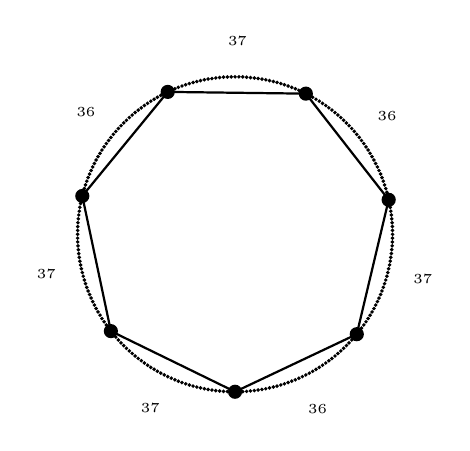
\begin{tikzpicture}[x=1mm, y=1mm]
    \fill (0,-20) circle[radius=0.25];
    \fill (0.49,-19.99) circle[radius=0.25];
    \fill (0.98,-19.98) circle[radius=0.25];
    \fill (1.47,-19.95) circle[radius=0.25];
    \fill (1.96,-19.9) circle[radius=0.25];
    \fill (2.45,-19.85) circle[radius=0.25];
    \fill (2.93,-19.78) circle[radius=0.25];
    \fill (3.42,-19.71) circle[radius=0.25];
    \fill (3.9,-19.62) circle[radius=0.25];
    \fill (4.38,-19.51) circle[radius=0.25];
    \fill (4.86,-19.4) circle[radius=0.25];
    \fill (5.33,-19.28) circle[radius=0.25];
    \fill (5.81,-19.14) circle[radius=0.25];
    \fill (6.27,-18.99) circle[radius=0.25];
    \fill (6.74,-18.83) circle[radius=0.25];
    \fill (7.2,-18.66) circle[radius=0.25];
    \fill (7.65,-18.48) circle[radius=0.25];
    \fill (8.1,-18.28) circle[radius=0.25];
    \fill (8.55,-18.08) circle[radius=0.25];
    \fill (8.99,-17.86) circle[radius=0.25];
    \fill (9.43,-17.64) circle[radius=0.25];
    \fill (9.86,-17.4) circle[radius=0.25];
    \fill (10.28,-17.15) circle[radius=0.25];
    \fill (10.7,-16.9) circle[radius=0.25];
    \fill (11.11,-16.63) circle[radius=0.25];
    \fill (11.52,-16.35) circle[radius=0.25];
    \fill (11.91,-16.06) circle[radius=0.25];
    \fill (12.3,-15.77) circle[radius=0.25];
    \fill (12.69,-15.46) circle[radius=0.25];
    \fill (13.06,-15.14) circle[radius=0.25];
    \fill (13.43,-14.82) circle[radius=0.25];
    \fill (13.79,-14.48) circle[radius=0.25];
    \fill (14.14,-14.14) circle[radius=0.25];
    \fill (14.48,-13.79) circle[radius=0.25];
    \fill (14.82,-13.43) circle[radius=0.25];
    \fill (15.14,-13.06) circle[radius=0.25];
    \fill (15.46,-12.69) circle[radius=0.25];
    \fill (15.77,-12.3) circle[radius=0.25];
    \fill (16.06,-11.91) circle[radius=0.25];
    \fill (16.35,-11.52) circle[radius=0.25];
    \fill (16.63,-11.11) circle[radius=0.25];
    \fill (16.9,-10.7) circle[radius=0.25];
    \fill (17.15,-10.28) circle[radius=0.25];
    \fill (17.4,-9.86) circle[radius=0.25];
    \fill (17.64,-9.43) circle[radius=0.25];
    \fill (17.86,-8.99) circle[radius=0.25];
    \fill (18.08,-8.55) circle[radius=0.25];
    \fill (18.28,-8.1) circle[radius=0.25];
    \fill (18.48,-7.65) circle[radius=0.25];
    \fill (18.66,-7.2) circle[radius=0.25];
    \fill (18.83,-6.74) circle[radius=0.25];
    \fill (18.99,-6.27) circle[radius=0.25];
    \fill (19.14,-5.81) circle[radius=0.25];
    \fill (19.28,-5.33) circle[radius=0.25];
    \fill (19.4,-4.86) circle[radius=0.25];
    \fill (19.51,-4.38) circle[radius=0.25];
    \fill (19.62,-3.9) circle[radius=0.25];
    \fill (19.71,-3.42) circle[radius=0.25];
    \fill (19.78,-2.93) circle[radius=0.25];
    \fill (19.85,-2.45) circle[radius=0.25];
    \fill (19.9,-1.96) circle[radius=0.25];
    \fill (19.95,-1.47) circle[radius=0.25];
    \fill (19.98,-0.98) circle[radius=0.25];
    \fill (19.99,-0.49) circle[radius=0.25];
    \fill (20,0) circle[radius=0.25];
    \fill (19.99,0.49) circle[radius=0.25];
    \fill (19.98,0.98) circle[radius=0.25];
    \fill (19.95,1.47) circle[radius=0.25];
    \fill (19.9,1.96) circle[radius=0.25];
    \fill (19.85,2.45) circle[radius=0.25];
    \fill (19.78,2.93) circle[radius=0.25];
    \fill (19.71,3.42) circle[radius=0.25];
    \fill (19.62,3.9) circle[radius=0.25];
    \fill (19.51,4.38) circle[radius=0.25];
    \fill (19.4,4.86) circle[radius=0.25];
    \fill (19.28,5.33) circle[radius=0.25];
    \fill (19.14,5.81) circle[radius=0.25];
    \fill (18.99,6.27) circle[radius=0.25];
    \fill (18.83,6.74) circle[radius=0.25];
    \fill (18.66,7.2) circle[radius=0.25];
    \fill (18.48,7.65) circle[radius=0.25];
    \fill (18.28,8.1) circle[radius=0.25];
    \fill (18.08,8.55) circle[radius=0.25];
    \fill (17.86,8.99) circle[radius=0.25];
    \fill (17.64,9.43) circle[radius=0.25];
    \fill (17.4,9.86) circle[radius=0.25];
    \fill (17.15,10.28) circle[radius=0.25];
    \fill (16.9,10.7) circle[radius=0.25];
    \fill (16.63,11.11) circle[radius=0.25];
    \fill (16.35,11.52) circle[radius=0.25];
    \fill (16.06,11.91) circle[radius=0.25];
    \fill (15.77,12.3) circle[radius=0.25];
    \fill (15.46,12.69) circle[radius=0.25];
    \fill (15.14,13.06) circle[radius=0.25];
    \fill (14.82,13.43) circle[radius=0.25];
    \fill (14.48,13.79) circle[radius=0.25];
    \fill (14.14,14.14) circle[radius=0.25];
    \fill (13.79,14.48) circle[radius=0.25];
    \fill (13.43,14.82) circle[radius=0.25];
    \fill (13.06,15.14) circle[radius=0.25];
    \fill (12.69,15.46) circle[radius=0.25];
    \fill (12.3,15.77) circle[radius=0.25];
    \fill (11.91,16.06) circle[radius=0.25];
    \fill (11.52,16.35) circle[radius=0.25];
    \fill (11.11,16.63) circle[radius=0.25];
    \fill (10.7,16.9) circle[radius=0.25];
    \fill (10.28,17.15) circle[radius=0.25];
    \fill (9.86,17.4) circle[radius=0.25];
    \fill (9.43,17.64) circle[radius=0.25];
    \fill (8.99,17.86) circle[radius=0.25];
    \fill (8.55,18.08) circle[radius=0.25];
    \fill (8.1,18.28) circle[radius=0.25];
    \fill (7.65,18.48) circle[radius=0.25];
    \fill (7.2,18.66) circle[radius=0.25];
    \fill (6.74,18.83) circle[radius=0.25];
    \fill (6.27,18.99) circle[radius=0.25];
    \fill (5.81,19.14) circle[radius=0.25];
    \fill (5.33,19.28) circle[radius=0.25];
    \fill (4.86,19.4) circle[radius=0.25];
    \fill (4.38,19.51) circle[radius=0.25];
    \fill (3.9,19.62) circle[radius=0.25];
    \fill (3.42,19.71) circle[radius=0.25];
    \fill (2.93,19.78) circle[radius=0.25];
    \fill (2.45,19.85) circle[radius=0.25];
    \fill (1.96,19.9) circle[radius=0.25];
    \fill (1.47,19.95) circle[radius=0.25];
    \fill (0.98,19.98) circle[radius=0.25];
    \fill (0.49,19.99) circle[radius=0.25];
    \fill (0,20) circle[radius=0.25];
    \fill (-0.49,19.99) circle[radius=0.25];
    \fill (-0.98,19.98) circle[radius=0.25];
    \fill (-1.47,19.95) circle[radius=0.25];
    \fill (-1.96,19.9) circle[radius=0.25];
    \fill (-2.45,19.85) circle[radius=0.25];
    \fill (-2.93,19.78) circle[radius=0.25];
    \fill (-3.42,19.71) circle[radius=0.25];
    \fill (-3.9,19.62) circle[radius=0.25];
    \fill (-4.38,19.51) circle[radius=0.25];
    \fill (-4.86,19.4) circle[radius=0.25];
    \fill (-5.33,19.28) circle[radius=0.25];
    \fill (-5.81,19.14) circle[radius=0.25];
    \fill (-6.27,18.99) circle[radius=0.25];
    \fill (-6.74,18.83) circle[radius=0.25];
    \fill (-7.2,18.66) circle[radius=0.25];
    \fill (-7.65,18.48) circle[radius=0.25];
    \fill (-8.1,18.28) circle[radius=0.25];
    \fill (-8.55,18.08) circle[radius=0.25];
    \fill (-8.99,17.86) circle[radius=0.25];
    \fill (-9.43,17.64) circle[radius=0.25];
    \fill (-9.86,17.4) circle[radius=0.25];
    \fill (-10.28,17.15) circle[radius=0.25];
    \fill (-10.7,16.9) circle[radius=0.25];
    \fill (-11.11,16.63) circle[radius=0.25];
    \fill (-11.52,16.35) circle[radius=0.25];
    \fill (-11.91,16.06) circle[radius=0.25];
    \fill (-12.3,15.77) circle[radius=0.25];
    \fill (-12.69,15.46) circle[radius=0.25];
    \fill (-13.06,15.14) circle[radius=0.25];
    \fill (-13.43,14.82) circle[radius=0.25];
    \fill (-13.79,14.48) circle[radius=0.25];
    \fill (-14.14,14.14) circle[radius=0.25];
    \fill (-14.48,13.79) circle[radius=0.25];
    \fill (-14.82,13.43) circle[radius=0.25];
    \fill (-15.14,13.06) circle[radius=0.25];
    \fill (-15.46,12.69) circle[radius=0.25];
    \fill (-15.77,12.3) circle[radius=0.25];
    \fill (-16.06,11.91) circle[radius=0.25];
    \fill (-16.35,11.52) circle[radius=0.25];
    \fill (-16.63,11.11) circle[radius=0.25];
    \fill (-16.9,10.7) circle[radius=0.25];
    \fill (-17.15,10.28) circle[radius=0.25];
    \fill (-17.4,9.86) circle[radius=0.25];
    \fill (-17.64,9.43) circle[radius=0.25];
    \fill (-17.86,8.99) circle[radius=0.25];
    \fill (-18.08,8.55) circle[radius=0.25];
    \fill (-18.28,8.1) circle[radius=0.25];
    \fill (-18.48,7.65) circle[radius=0.25];
    \fill (-18.66,7.2) circle[radius=0.25];
    \fill (-18.83,6.74) circle[radius=0.25];
    \fill (-18.99,6.27) circle[radius=0.25];
    \fill (-19.14,5.81) circle[radius=0.25];
    \fill (-19.28,5.33) circle[radius=0.25];
    \fill (-19.4,4.86) circle[radius=0.25];
    \fill (-19.51,4.38) circle[radius=0.25];
    \fill (-19.62,3.9) circle[radius=0.25];
    \fill (-19.71,3.42) circle[radius=0.25];
    \fill (-19.78,2.93) circle[radius=0.25];
    \fill (-19.85,2.45) circle[radius=0.25];
    \fill (-19.9,1.96) circle[radius=0.25];
    \fill (-19.95,1.47) circle[radius=0.25];
    \fill (-19.98,0.98) circle[radius=0.25];
    \fill (-19.99,0.49) circle[radius=0.25];
    \fill (-20,0) circle[radius=0.25];
    \fill (-19.99,-0.49) circle[radius=0.25];
    \fill (-19.98,-0.98) circle[radius=0.25];
    \fill (-19.95,-1.47) circle[radius=0.25];
    \fill (-19.9,-1.96) circle[radius=0.25];
    \fill (-19.85,-2.45) circle[radius=0.25];
    \fill (-19.78,-2.93) circle[radius=0.25];
    \fill (-19.71,-3.42) circle[radius=0.25];
    \fill (-19.62,-3.9) circle[radius=0.25];
    \fill (-19.51,-4.38) circle[radius=0.25];
    \fill (-19.4,-4.86) circle[radius=0.25];
    \fill (-19.28,-5.33) circle[radius=0.25];
    \fill (-19.14,-5.81) circle[radius=0.25];
    \fill (-18.99,-6.27) circle[radius=0.25];
    \fill (-18.83,-6.74) circle[radius=0.25];
    \fill (-18.66,-7.2) circle[radius=0.25];
    \fill (-18.48,-7.65) circle[radius=0.25];
    \fill (-18.28,-8.1) circle[radius=0.25];
    \fill (-18.08,-8.55) circle[radius=0.25];
    \fill (-17.86,-8.99) circle[radius=0.25];
    \fill (-17.64,-9.43) circle[radius=0.25];
    \fill (-17.4,-9.86) circle[radius=0.25];
    \fill (-17.15,-10.28) circle[radius=0.25];
    \fill (-16.9,-10.7) circle[radius=0.25];
    \fill (-16.63,-11.11) circle[radius=0.25];
    \fill (-16.35,-11.52) circle[radius=0.25];
    \fill (-16.06,-11.91) circle[radius=0.25];
    \fill (-15.77,-12.3) circle[radius=0.25];
    \fill (-15.46,-12.69) circle[radius=0.25];
    \fill (-15.14,-13.06) circle[radius=0.25];
    \fill (-14.82,-13.43) circle[radius=0.25];
    \fill (-14.48,-13.79) circle[radius=0.25];
    \fill (-14.14,-14.14) circle[radius=0.25];
    \fill (-13.79,-14.48) circle[radius=0.25];
    \fill (-13.43,-14.82) circle[radius=0.25];
    \fill (-13.06,-15.14) circle[radius=0.25];
    \fill (-12.69,-15.46) circle[radius=0.25];
    \fill (-12.3,-15.77) circle[radius=0.25];
    \fill (-11.91,-16.06) circle[radius=0.25];
    \fill (-11.52,-16.35) circle[radius=0.25];
    \fill (-11.11,-16.63) circle[radius=0.25];
    \fill (-10.7,-16.9) circle[radius=0.25];
    \fill (-10.28,-17.15) circle[radius=0.25];
    \fill (-9.86,-17.4) circle[radius=0.25];
    \fill (-9.43,-17.64) circle[radius=0.25];
    \fill (-8.99,-17.86) circle[radius=0.25];
    \fill (-8.55,-18.08) circle[radius=0.25];
    \fill (-8.1,-18.28) circle[radius=0.25];
    \fill (-7.65,-18.48) circle[radius=0.25];
    \fill (-7.2,-18.66) circle[radius=0.25];
    \fill (-6.74,-18.83) circle[radius=0.25];
    \fill (-6.27,-18.99) circle[radius=0.25];
    \fill (-5.81,-19.14) circle[radius=0.25];
    \fill (-5.33,-19.28) circle[radius=0.25];
    \fill (-4.86,-19.4) circle[radius=0.25];
    \fill (-4.38,-19.51) circle[radius=0.25];
    \fill (-3.9,-19.62) circle[radius=0.25];
    \fill (-3.42,-19.71) circle[radius=0.25];
    \fill (-2.93,-19.78) circle[radius=0.25];
    \fill (-2.45,-19.85) circle[radius=0.25];
    \fill (-1.96,-19.9) circle[radius=0.25];
    \fill (-1.47,-19.95) circle[radius=0.25];
    \fill (-0.98,-19.98) circle[radius=0.25];
    \fill (-0.49,-19.99) circle[radius=0.25];
    \draw[thick] (0,-20) -- (15.46,-12.69) -- (19.51,4.38) -- (8.99,17.86) -- (-8.55,18.08) -- (-19.4,4.86) -- (-15.77,-12.3) -- cycle;
    \fill (0,-20) circle[radius=0.9];
    \fill (15.46,-12.69) circle[radius=0.9];
    \fill (19.51,4.38) circle[radius=0.9];
    \fill (8.99,17.86) circle[radius=0.9];
    \fill (-8.55,18.08) circle[radius=0.9];
    \fill (-19.4,4.86) circle[radius=0.9];
    \fill (-15.77,-12.3) circle[radius=0.9];
    \node[font=\tiny] at (10.48,-22.15) {36};
    \node[font=\tiny] at (23.84,-5.66) {37};
    \node[font=\tiny] at (19.31,15.07) {36};
    \node[font=\tiny] at (0.3,24.5) {37};
    \node[font=\tiny] at (-18.94,15.54) {36};
    \node[font=\tiny] at (-23.97,-5.07) {37};
    \node[font=\tiny] at (-10.75,-22.02) {37};
    \end{tikzpicture}
  \end{minipage}%
  \begin{minipage}[c]{0.5\linewidth}
    An $n$-color palette takes every $\frac{256}{n}$-th vertex, in whole
    steps spread Bresenham's way \cite{bresenham}: with $256 = qn + s$,
    \[ n - s \text{ gaps of } q, \qquad s \text{ gaps of } q + 1. \]
    For $n = 7$: 3 gaps of 36 and 4 of 37.
    Its 256 rotations are \texttt{generatePalettes(7)}.
  \end{minipage}
\end{slide}

\begin{slide}{Twelve colors at four lightnesses}
  \centering
  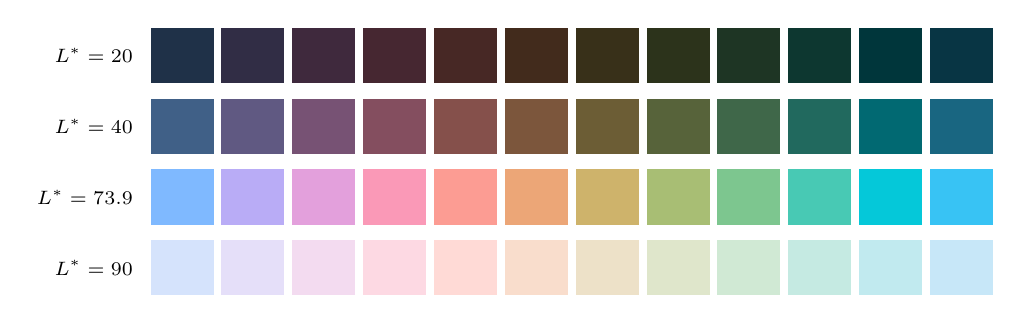
\begin{tikzpicture}[x=1mm, y=1mm]
    \node[left, font=\scriptsize] at (-1,3.5) {$L^* = 20$};
    \fill[color={rgb,255:red,31;green,49;blue,72}] (0,0) rectangle +(8,7);
    \fill[color={rgb,255:red,49;green,45;blue,69}] (9,0) rectangle +(8,7);
    \fill[color={rgb,255:red,63;green,41;blue,61}] (18,0) rectangle +(8,7);
    \fill[color={rgb,255:red,70;green,39;blue,49}] (27,0) rectangle +(8,7);
    \fill[color={rgb,255:red,71;green,40;blue,37}] (36,0) rectangle +(8,7);
    \fill[color={rgb,255:red,66;green,43;blue,28}] (45,0) rectangle +(8,7);
    \fill[color={rgb,255:red,56;green,48;blue,25}] (54,0) rectangle +(8,7);
    \fill[color={rgb,255:red,44;green,51;blue,27}] (63,0) rectangle +(8,7);
    \fill[color={rgb,255:red,30;green,53;blue,36}] (72,0) rectangle +(8,7);
    \fill[color={rgb,255:red,13;green,55;blue,48}] (81,0) rectangle +(8,7);
    \fill[color={rgb,255:red,0;green,54;blue,59}] (90,0) rectangle +(8,7);
    \fill[color={rgb,255:red,8;green,53;blue,68}] (99,0) rectangle +(8,7);
    \node[left, font=\scriptsize] at (-1,-5.5) {$L^* = 40$};
    \fill[color={rgb,255:red,64;green,96;blue,135}] (0,-9) rectangle +(8,7);
    \fill[color={rgb,255:red,96;green,89;blue,130}] (9,-9) rectangle +(8,7);
    \fill[color={rgb,255:red,119;green,82;blue,116}] (18,-9) rectangle +(8,7);
    \fill[color={rgb,255:red,132;green,78;blue,95}] (27,-9) rectangle +(8,7);
    \fill[color={rgb,255:red,133;green,80;blue,75}] (36,-9) rectangle +(8,7);
    \fill[color={rgb,255:red,124;green,86;blue,60}] (45,-9) rectangle +(8,7);
    \fill[color={rgb,255:red,108;green,93;blue,53}] (54,-9) rectangle +(8,7);
    \fill[color={rgb,255:red,87;green,99;blue,58}] (63,-9) rectangle +(8,7);
    \fill[color={rgb,255:red,63;green,103;blue,73}] (72,-9) rectangle +(8,7);
    \fill[color={rgb,255:red,33;green,105;blue,94}] (81,-9) rectangle +(8,7);
    \fill[color={rgb,255:red,1;green,105;blue,114}] (90,-9) rectangle +(8,7);
    \fill[color={rgb,255:red,25;green,102;blue,129}] (99,-9) rectangle +(8,7);
    \node[left, font=\scriptsize] at (-1,-14.5) {$L^* = 73.9$};
    \fill[color={rgb,255:red,127;green,185;blue,255}] (0,-18) rectangle +(8,7);
    \fill[color={rgb,255:red,185;green,172;blue,246}] (9,-18) rectangle +(8,7);
    \fill[color={rgb,255:red,227;green,160;blue,220}] (18,-18) rectangle +(8,7);
    \fill[color={rgb,255:red,250;green,153;blue,183}] (27,-18) rectangle +(8,7);
    \fill[color={rgb,255:red,252;green,156;blue,147}] (36,-18) rectangle +(8,7);
    \fill[color={rgb,255:red,236;green,166;blue,119}] (45,-18) rectangle +(8,7);
    \fill[color={rgb,255:red,206;green,179;blue,107}] (54,-18) rectangle +(8,7);
    \fill[color={rgb,255:red,168;green,190;blue,116}] (63,-18) rectangle +(8,7);
    \fill[color={rgb,255:red,125;green,198;blue,143}] (72,-18) rectangle +(8,7);
    \fill[color={rgb,255:red,72;green,201;blue,180}] (81,-18) rectangle +(8,7);
    \fill[color={rgb,255:red,5;green,200;blue,217}] (90,-18) rectangle +(8,7);
    \fill[color={rgb,255:red,56;green,195;blue,244}] (99,-18) rectangle +(8,7);
    \node[left, font=\scriptsize] at (-1,-23.5) {$L^* = 90$};
    \fill[color={rgb,255:red,213;green,227;blue,252}] (0,-27) rectangle +(8,7);
    \fill[color={rgb,255:red,229;green,223;blue,249}] (9,-27) rectangle +(8,7);
    \fill[color={rgb,255:red,243;green,219;blue,240}] (18,-27) rectangle +(8,7);
    \fill[color={rgb,255:red,253;green,217;blue,227}] (27,-27) rectangle +(8,7);
    \fill[color={rgb,255:red,255;green,218;blue,214}] (36,-27) rectangle +(8,7);
    \fill[color={rgb,255:red,249;green,221;blue,204}] (45,-27) rectangle +(8,7);
    \fill[color={rgb,255:red,237;green,225;blue,200}] (54,-27) rectangle +(8,7);
    \fill[color={rgb,255:red,223;green,230;blue,203}] (63,-27) rectangle +(8,7);
    \fill[color={rgb,255:red,208;green,233;blue,212}] (72,-27) rectangle +(8,7);
    \fill[color={rgb,255:red,197;green,234;blue,226}] (81,-27) rectangle +(8,7);
    \fill[color={rgb,255:red,193;green,234;blue,239}] (90,-27) rectangle +(8,7);
    \fill[color={rgb,255:red,199;green,231;blue,248}] (99,-27) rectangle +(8,7);
  \end{tikzpicture}

  \texttt{generatePalettes(12, \{ lightness \})[0]}: one hue circle, four
  lightnesses. Within a row, every swatch has the same luminance.
\end{slide}

\begin{slide}{When colors collide}
  \begin{minipage}[c]{0.48\linewidth}
    Near black and white the 256-gon is small, and 8-bit sRGB rounds some
    vertices to the same color. A lightness then uses its largest $n$-gon
    whose colors are all distinct.
  \end{minipage}\hfill
  \begin{minipage}[c]{0.46\linewidth}
    \centering
    \begin{tabular}{rrr}
      \toprule
      $L^*$ & $r(L^*)$ & largest unique $n$ \\
      \midrule
    1 & 1.281 & 21 \\
    5 & 6.403 & 63 \\
    10 & 11.614 & 93 \\
    20 & 16.091 & 133 \\
    40 & 25.030 & 225 \\
    73.9124 & 40.188 & 256 \\
    85 & 21.504 & 179 \\
    95 & 6.639 & 86 \\
    99 & 1.290 & 18 \\
      \bottomrule
    \end{tabular}
  \end{minipage}
\end{slide}

\begin{slide}{Mapping colors onto a palette}
  \texttt{mapColors} takes $n$ colors to the nearest $n$-color palette.
  \begin{enumerate}
    \item Project each color to its $(a^*, b^*)$ on the lightness's plane.
    \item For each of the 256 rotations, the cost of color $i$ taking vertex
      $j$ is their distance,
      \[ d_{ij} = \sqrt{(a_i - a_j)^2 + (b_i - b_j)^2}. \]
    \item The Hungarian method \cite{kuhn, munkres} finds the assignment of
      least total cost in $O(n^3)$.
    \item The rotation with the least cost wins.
  \end{enumerate}
\end{slide}

\begin{slide}{Text on a palette}
  WCAG's contrast ratio \cite{wcag} between luminances $Y_1 > Y_2$ is
  \[ \frac{Y_1 + 0.05}{Y_2 + 0.05}. \]
  Every color at one $L^*$ shares its $Y$, so one text color fits them all:
  black wins where
  \[ \frac{Y + 0.05}{0.05} \ \ge\ \frac{1.05}{Y + 0.05}
     \iff Y \ge \sqrt{0.0525} - 0.05 \approx 0.179, \]
  that is, $L^* \gtrsim 49.4$. Below it, white.
\end{slide}

\begin{slide}{References}
  \nocite{*}
  \bibliographystyle{plain}
  \small
  \bibliography{nicrainha}
\end{slide}
\end{document}
